\documentclass[galaxies,article,submit,moreauthors,pdftex,10pt,a4paper]{mdpi}

% TODO:
% - Mention Hercules-Aquila somewhere as a genuine "shell" candidate

\usepackage{amsmath}
\usepackage{amssymb}
\usepackage{aas_macros}

% -------------------
% Some useful macros:
% -------------------

% Formatting:
\newcommand{\project}[1]{\textsl{#1}}
\newcommand{\survey}[1]{\textsl{#1}}
\newcommand{\acronym}[1]{{\small{#1}}}
\newcommand{\apogee}{\survey{\acronym{APOGEE}}}
\newcommand{\sdssiii}{\survey{\acronym{SDSS-III}}}

% Math:
\newcommand{\kpc}{\mathrm{kpc}}
\newcommand{\msun}{\mathrm{M}_\odot}
\newcommand{\kms}{\mathrm{km}~\mathrm{s}^{-1}}
\newcommand{\frrmg}{\ensuremath{f_{\rm RR:MG}}}

\newcommand{\ion}[2]{#1\,\textsc{#2}}

%--------------------
% Class Options:
%--------------------
% journal
%----------
% Choose between the following MDPI journals:
% actuators, admsci, aerospace, agriculture, agronomy, algorithms, animals, antibiotics, antibodies, antioxidants, applsci, arts, atmosphere, atoms, axioms, batteries, bdcc, behavsci, beverages, bioengineering, biology, biomedicines, biomimetics, biomolecules, biosensors, brainsci, buildings, carbon, cancers, catalysts, cells, challenges, chemengineering, chemosensors, children, chromatography, climate, coatings, computation, computers, condensedmatter, cosmetics, cryptography, crystals, data, dentistry, designs, diagnostics, diseases, diversity, econometrics, economies, education, electronics, energies, entropy, environments, epigenomes, fermentation, fibers, fishes, fluids, foods, forests, fractalfract, futureinternet, galaxies, games, gastrointestdisord, gels, genealogy, genes, geosciences, geriatrics, healthcare, horticulturae, humanities, hydrology, informatics, information, infrastructures, inorganics, insects, instruments, ijerph, ijfs, ijms, ijgi, ijtpp, inventions, jcdd, jcm, jcs, jdb, jfb, jfmk, jimaging, jof, jintelligence, jlpea, jmmp, jmse, jpm, jrfm, jsan, land, languages, laws, life, literature, logistics, lubricants, machines, magnetochemistry, marinedrugs, materials, mathematics, mca, mti, medsci, medicines, membranes, metabolites, metals, microarrays, micromachines, microorganisms, minerals, molbank, molecules, mps, nanomaterials, ncrna, neonatalscreening, nitrogen, nutrients, ohbm, particles, pathogens, pharmaceuticals, pharmaceutics, pharmacy, philosophies, photonics, plants, polymers, proceedings, processes, proteomes, publications, quaternary, qubs, recycling, religions, remotesensing, resources, risks, robotics, safety, scipharm, sensors, separations, sexes, sinusitis, socsci, societies, soilprocesses, soils, sports, standards, sustainability, symmetry, systems, technologies, toxics, toxins, tropicalmed, universe, urbansci, vaccines, vetsci, viruses, vision, water
%---------
% article
%---------
% The default type of manuscript is article, but can be replaced by:
% addendum, article, benchmark, book, bookreview, briefreport, casereport, changes, comment, commentary, communication, conceptpaper, correction, conferenceproceedings, conferencereport, expressionofconcern, meetingreport, creative, datadescriptor, discussion, editorial, essay, erratum, hypothesis, interestingimage, letter, newbookreceived, opinion, obituary, projectreport, reply, reprint, retraction, review, perspective, preprints, protocol, shortnote, supfile, technicalnote, viewpoint
% supfile = supplementary materials
%----------
% submit
%----------
% The class option "submit" will be changed to "accept" by the Editorial Office when the paper is accepted. This will only make changes to the frontpage (e.g. the logo of the journal will get visible), the headings, and the copyright information. Also, line numbering will be removed. Journal info and pagination for accepted papers will also be assigned by the Editorial Office.
%------------------
% moreauthors
%------------------
% If there is only one author the class option oneauthor should be used. Otherwise use the class option moreauthors.
%---------
% pdftex
%---------
% The option pdftex is for use with pdfLaTeX. If eps figure are used, remove the option pdftex and use LaTeX and dvi2pdf.

%=================================================================
\firstpage{1}
\makeatletter
\setcounter{page}{\@firstpage}
\makeatother
\articlenumber{x}
\doinum{10.3390/------}
\pubvolume{xx}
\pubyear{2017}
\copyrightyear{2017}
\externaleditor{Academic Editor: name}
\history{Received: date; Accepted: date; Published: date}

%------------------------------------------------------------------
% The following line should be uncommented if the LaTeX file is uploaded to arXiv.org
%\pdfoutput=1

%=================================================================
% Add packages and commands here. The following packages are loaded in our class file: fontenc, calc, indentfirst, fancyhdr, graphicx, lastpage, ifthen, lineno, float, amsmath, setspace, enumitem, mathpazo, booktabs, titlesec, etoolbox, amsthm, hyphenat, natbib, hyperref, footmisc, geometry, caption, url, mdframed, tabto, soul, multirow, microtype

%=================================================================
%% Please use the following mathematics environments: Theorem, Lemma, Corollary, Proposition, Characterization, Property, Problem, Example, ExamplesandDefinitions, Hypothesis, Remark, Definition
%% For proofs, please use the proof environment (the amsthm package is loaded by the MDPI class).

%=================================================================
% Full title of the paper (Capitalized)
\Title{Disk Heating, Galactoseismology, and the Formation of Stellar Halos}

% If this is an expanded version of a conference paper, please cite it here: enter the full citation of your conference paper, and add $^\dagger$ in the end of the title of this article.
%\conference{Title}

% Authors, for the paper (add full first names)
\Author{Kathryn V. Johnston $^{1,\dagger}$, Adrian M. Price-Whelan$^{2,\dagger}$, Maria Bergemann$^{3}$, Chervin Laporte$^{1}$, Ting S. Li$^{4}$, Allyson A. Sheffield$^{5}$, Branimir Sesar$^{3}$, and Sanjib Sharma $^{6}$}
% Rachel Beaton? Steve Majewski? Sanjib Sharma?

% Authors, for metadata in PDF
\AuthorNames{Firstname Lastname, Firstname Lastname and Firstname Lastname}

% Affiliations / Addresses (Add [1] after \address if there is only one affiliation.)
\address{
$^{1}$ \quad Department of Astronomy, Columbia University \\
$^{2}$ \quad Department of Astrophysical Sciences, Princeton University \\
$^{3}$ \quad Max Planck Institute for Astronomy, Heidelberg\\
$^{4}$ \quad Department of Physics \& Astronomy, Texas A \& M University\\
$^{5}$ \quad City University of New York, LaGuardia Community College \\
$^{6}$ \quad Sydney Institute for Astronomy, School of Physics, University of Sydney \\
}

% Contact information of the corresponding author
\corres{Correspondence: kvj@astro.columbia.edu; Tel.: +1-212-854-3884}

% Current address and/or shared authorship
%\firstnote{Current address: Affiliation 3}
\firstnote{These authors contributed equally to this work.}
% The commands \thirdnote{} till \eighthnote{} are available for further notes

% Simple summary
%\simplesumm{}

% Abstract (Do not use inserted blank lines, i.e. \\)
\abstract{
%A single paragraph of about 200 words maximum. 1) Background: Place the question addressed in a broad context and highlight the purpose of the study; 2) Methods: Describe briefly the main methods or treatments applied; 3) Results: Summarize the article's main findings; and 4) Conclusion: Indicate the main conclusions or interpretations. The abstract should be an objective representation of the article, it must not contain results which are not presented and substantiated in the main text and should not exaggerate the main conclusions.
Deep photometric surveys of the Milky Way have revealed diffuse structures
encircling our Galaxy in regions far beyond the ``classical'' end of the
stellar disk.
This article reviews results from our own and other observational programs, which together suggest that, despite their extreme positions, the stars in these structures were nevertheless formed in our Galactic disk.
Mounting evidence from recent observations and simulations implies kinematic connections between several of these distinct structures.
This suggests the existence of collective disk oscillations that can plausibly be traced all the way to asymmetries seen in the stellar velocity distribution around the Sun.
There are multiple interesting implications of these findings:
they promise new perspectives on the process of disk heating;
they provide direct evidence for a stellar halo formation mechanism in addition to the accretion and disruption of satellite galaxies; and,
they motivate searches of current and near-future surveys to trace these oscillations across the Galaxy.
Such maps could be used as dynamical diagnostics in the emerging field of ``Galactoseismology,'' which promises to model the history of interactions between the Milky Way and its entourage of satellites, as well examine the density of our dark matter halo.
As sensitivity to very low surface brightness features around external galaxies increases, many more examples of such disk oscillations will likely be identified.
Statistical samples of such features not only encode detailed information about
interaction rates and mergers, but also about long sought-after dark matter
halo densities and shapes.
Models for the Milky Way's own Galactoseismic history will therefore serve as a
critical foundation for studying the weak interactions of galaxies across the
universe.
}

% Keywords
\keyword{galaxy formation; galactic disks; stellar halos; Milky Way.}

% The fields PACS, MSC, and JEL may be left empty or commented out if not applicable
%\PACS{J0101}
%\MSC{}
%\JEL{}

%%%%%%%%%%%%%%%%%%%%%%%%%%%%%%%%%%%%%%%%%%
% Only for journal Applied Sciences:
%\featuredapplication{Authors are encouraged to provide a concise description of the specific application or a potential application of the work. This section is not mandatory.}
%%%%%%%%%%%%%%%%%%%%%%%%%%%%%%%%%%%%%%%%%%


%%%%%%%%%%%%%%%%%%%%%%%%%%%%%%%%%%%%%%%%%%
% Only for the journal Data:
%\dataset{DOI number or link to the deposited data set in cases where the data set is published or set to be published separately. If the data set is submitted and will be published as a supplement to this paper in the journal Data, this field will be filled by the editors of the journal. In this case, please make sure to submit the data set as a supplement when entering your manuscript into our manuscript editorial system.}

%\datasetlicense{license under which the data set is made available (CC0, CC-BY, CC-BY-SA, CC-BY-NC, etc.)}

%%%%%%%%%%%%%%%%%%%%%%%%%%%%%%%%%%%%%%%%%%
% For Conference Proceedings Papers:
%\conferencetitle{Add the conference title here}

%\setcounter{secnumdepth}{4}
%%%%%%%%%%%%%%%%%%%%%%%%%%%%%%%%%%%%%%%%%%

\begin{document}

%%%%%%%%%%%%%%%%%%%%%%%%%%%%%%%%%%%%%%%%%%

%%%%%%%%%%%%%%%%%%%%%%%%%%%%%%%%%%%%%%%%%%
%\setcounter{section}{-1} %% Remove this when starting to work on the template.

\section{Introduction}

Our perspective on the Milky Way presents both unique challenges and unique opportunities towards our quest to understand galaxies more generally.
From our position inside, it is the one galaxy in the Universe that we cannot take an image of but rather need to survey the entire sky in order to map its structure.
On the other hand, it is one of the few galaxies that we can presently study by individual stars and is the only one for which we can hope to make volume-complete maps of full-space positions and velocities for significant numbers of unevolved stars.
Present and recent sky surveys have already considerably advanced this effort, and near-future surveys will deliver massive datasets that will enable detailed studies of stellar structures throughout the Galactic volume.
%move beyond co-ordinates restricted to random projections in a limited number of directions to

% We are in the middle of a renaissance in Milky Way studies, fueled by stellar data sets of sufficient scope in terms of sky coverage and numbers to exploit our perspective as a strength rather than a liability
% %and take full advantage of our proximity
% to create vast catalogues of stellar data.

Emerging in the 1990's, the catalogues that inspired this recent acceleration not only mapped global structures in our Galaxy, but also revealed the ubiquity of substructure within it.
These revelations added an unforeseen richness to interpretations, and encouraged the development of new dynamical tools for studying ongoing interactions and formation histories:
\survey{Hipparcos} \cite{esa97} found moving groups of stars in the velocity distribution in the Solar Neighborhood \cite{dehnen98}, some corresponding (as expected) to destroyed stars clusters, while others (unexpectedly) could plausibly be explained as signatures of resonances with the Galactic bar \cite{dehnen00};
the Sloan Digital Sky Survey \cite[hereafter, SDSS ---][]{york00,stoughton02,abazajian03} found many streams of Main Sequence Turnoff (MSTO) stars in our stellar halo, thought to be from long-dead satellite galaxies and dissolved globular clusters \cite{newberg02,belokurov06} as a stunning confirmation that our Galaxy had indeed formed hierarchically \cite[e.g.][]{bullock01,bullock05};
and M giant stars selected from the Two Micron All Sky Survey \cite[hereafter, 2MASS ---][]{nikolaev00} traced the debris from the Sagittarius dwarf galaxy entirely around the Sky \cite{majewski03} to offer a window on the history of its disruption \cite{law10}.
From these and many other studies that use large survey catalogues, it is now clear that the Milky Way is full of kinematic substructure.

% APW COMMENT: this section makes it sound like the surveys discovered these
% things "for free," but really it was the authors you cite who found these
% things. I would rearrange to say, e.g., "Using data from the
% \survey{Hipparcos} mission \cite{esa97}, moving groups of stars were found
% in the velocity distribution in the Solar Neighborhood
% \cite{dehnen98}...etc"
% KVJ: will get to if there is time

\begin{figure}[!ht]
\label{fig:ting}
\centering
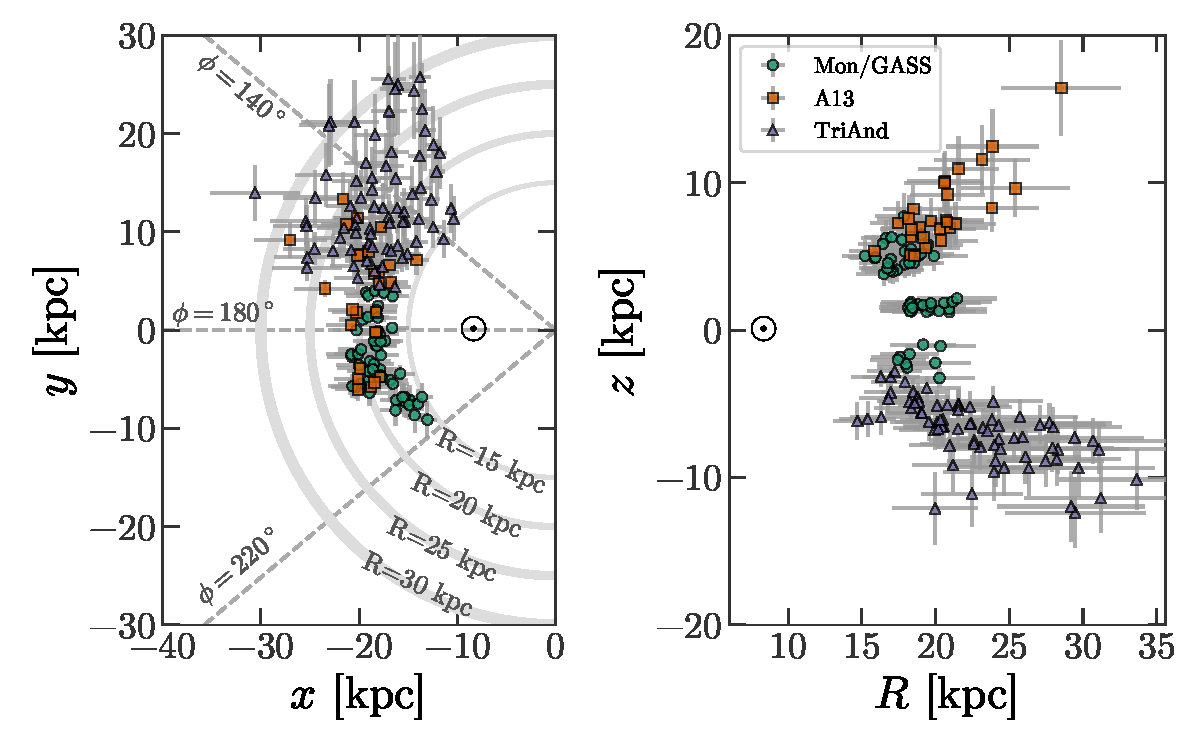
\includegraphics[width=6 in]{figures/xy_Rz.pdf}
\caption{\label{fig:ting}
Summary of the spatial distribution of M giants in each of the three
low-latitude structures.
Note that at lower Galactic latitudes, the lack of candidate M giant members is
due to selection effects and crowding near the midplane; we expect the
structures to continue towards even lower latitudes, but blend with ordinary
disk stars.
Markers represent individual stars identified as likely members of each of the
three structures discussed in this work (see figure legend).
Distance estimates come from photometric alone and have expected absolute
uncertainties around $\approx$20\% for TriAnd and A13 \cite{sheffield14,li17}
and $\approx$25\% for GASS.
Grey curves in left panel show Galactocentric circles with cylindrical radii,
$R$, indicated on the figure.
The position of the sun is marked with the solar symbol $\odot$.
}
\end{figure}

Figure~\ref{fig:ting}, reproduced from \cite{li17}, shows the spatial distribution of M giant stars associated with three such substructures that this paper concentrates on: the so-called Monoceros Ring, Triangulum-Andromeda clouds, and A13.
Each of these substructures were originally identified using SDSS and 2MASS photometry as over-densities in stellar number counts relative to the expected global structure of the disk or inner stellar halo.\footnote{Note that the same region on the sky has been shown to be richly structured on even smaller scales\cite{slater14,martin14,deason14} but we do not discuss these sub-substructures here.}
Unlike stellar streams, these substructures are present at a range of low to moderate Galactic latitudes --- we will hereafter refer to them collectively as the ``low-latitude structures''.
The following is a brief  summary of the discovery and initial follow-up papers that outlined their basic properties.
\begin{description}
\item{\it The Monoceros Ring or Giant Anticenter Stellar Structure} (hereafter Mon/GASS) is an arc- or ring-like feature of stars beyond the expected edge of the Galactic disk \cite[assumed to be $\approx 5~\kpc$ beyond the Sun in cylindrical radius ---][]{robin92}.
The feature spans a large area: Galactic longitudes $\approx 120^\circ \lesssim l \lesssim 240^\circ$, latitudes $-30^\circ \lesssim b \lesssim +40^\circ$, and Heliocentric distances $5\lesssim d_\odot \lesssim 10~\kpc$ (\cite{Morganson:2016}).
Mon/GASS was originally found as an excess of main sequence stars in SDSS \cite{yanny03,ibata03} and M giant stars in 2MASS \cite{rochapinto03}.
Follow-up spectra of the M giant stars indicate that they follow a clear trend in mean velocity with Galactic longitude with small dispersion \cite{crane03}.
\item{\it The Triangulum-Andromeda Clouds} (hereafter TriAnd 1 and TriAnd 2) were first discovered as a single diffuse over-density of M giant stars covering the area $\approx 100^\circ \lesssim l \lesssim 150^\circ$, $\approx 20^\circ \lesssim b \lesssim 40^\circ$ overlapping the Mon/GASS structure on the sky but at larger Heliocentric distances of approximately $15$--$30~\kpc$ \cite{rochapinto04}.
Follow-up spectroscopy showed that the M giants exhibit a coherent velocity sequence with a small dispersion \cite{rochapinto04} and later deep photometry in the region revealed associated MSTO stars and an estimate of the surface brightness of the feature $\Sigma > 32~{\rm mag}~{\rm arcsec}^{-2}$ \cite{majewski04}.
Subsequent photometric work also revealed the presence of {\it two} distinct main sequences \cite{martin07}.
\item{\it A13} is another tenuous association of stars discovered by applying a group finding algorithm \cite{sharma09} to the catalogue of all 2MASS M giants \cite{sharma10}.
This group sits in the north Galactic hemisphere in the area $\approx 125^\circ \lesssim l \lesssim 210^\circ$, $\approx 20^\circ \lesssim b \lesssim 40^\circ$ and at approximate distances of $\approx 12$--$20~\kpc$.
\end{description}
We note that (1) these structures likely continue towards lower Galactic
latitudes ($b < 20^\circ$) but are incomplete due to Galactic extinction near
the midplane, and (2) each structure in reality has a longitude-dependent
distance dependence that is ignored in the quoted distance ranges above.
Many models have been proposed to explain the formation and existence of these
substructures.
Mon/GASS has been attributed to the accretion of a satellite on a retrograde orbit \cite{penarrubia05}, a natural extension of the Galactic warp \cite{momany04,momany06}, or disturbances to the Galactic disk \cite{kazantzidis08,younger08,purcell11,xu15,gomez16}.
For the TriAnd clouds, their extreme positions at $(R,Z) \approx (20, -8)~\kpc$ and $(R,Z) \approx (25, -10)~\kpc$,
%and $(R,Z) \approx (20, 8)~\kpc$
(across a large range in Galactocentric azimuth, $\phi$) seems to exclude a disturbed disk as a possible origin in these cases and a satellite on a retrograde orbit has again been shown to provide a plausible explanation of their structure \cite{sheffield14}.
Indeed, preliminary abundance studies show [$\alpha$/Fe] values for member M giants of both Mon/GASS and the TriAnd Clouds reminiscent of stars in Galactic satellites and unlike the disk \cite{chou2010b,chou11} --- see Section \ref{sec:abundances} for a more complete discussion.
% APW COMMENT: I found it strange that the historical context doesn't include
% our recent work - maybe we should state that this was the status before our
% group started working on follow-up, or something? Otherwise, GASS section
% should get a reference to upcoming Sheffield+(in prep.) paper on RR Lyrae,
% TriAnd section should get references to Sheffield+2014(?) and
% Price-Whelan+2015, A13 paper should get reference to Li+2017
% KVJ: hope sentence above helps?

A more convincing, coherent picture of the nature of these low-latitude structures is just beginning to emerge.
This paper reviews the contributions our own group has made to formulating this picture, which include spectroscopic surveys of the low-latitude structures to study metallicity and velocities \cite{sheffield14,li17}, stellar populations \cite{pricewhelan15}, and abundance patterns (paper currently in preparation, Bergemann et al 2017), as well as numerical simulations \cite{sheffield14,laporte16}.
We summarize this observational and theoretical work in Section 2 and 3 respectively, adding in the context of contemporary work from other groups, as well as the larger context of possible connections across the Galactic disk.
Armed with this understanding of the nature of these substructures, we go on in Section 4 to discuss prospects for mapping such structures more generally around our own and other Galaxies.
We end in Section 5 by outlining the motivation for making such maps, asking what they might be telling us about bigger questions: galaxy formation scenarios and dark matter distributions.

% APW COMMENT: I'm not sure about the subsection grouping below.  I'm wondering
% if there is another way to reorganize...Perhaps subsections for name of
% structure, subsubsections for "observational follow-up", "theoretical
% understanding", "future work needed"? i.e. take the transpose of what is here
% now, if you know what I mean.
% KVJ: not _sure_ I agree and no time to implement

\section{The Nature of Structures Around the Outer Disk --- Summary of Observations}
\label{sec:obs}

\subsection{Spectroscopic surveys}

From clustering in positions or distance alone, many candidate groups and
over-densities of M giants have been identified in the outer disk / inner halo.
Over the last five years our group has pursued a spectroscopic campaign to
follow up members of these candidate structure with the aims of (1) confirming
the existence of substructure in velocities, (2) measuring chemical abundances,
and (3) studying the constituent stellar populations.
These goals then inform our own efforts to produce plausible dynamical
formation scenarios using simulations.
We were interested in particular in {\it avoiding} the collimated stellar streams that have been well-studied in prior work \cite[such as Sgr, Orphan, GD1 and Pal 5 --- see, e.g.,][]{law10,koposov10,kuepper15,bovy16}
and instead considered groups that appeared as diffuse, amorphous, extended stellar structures such as TriAnd 1 and 2 \cite{rochapinto04} and A13 \cite{sharma10}.
Initial interpretations of these morphologies suggested the structures could be {\it shells} --- debris from the disruption of satellite galaxies on near-radial orbits \cite{johnston08} --- as seen from an internal perspective.

In our first results \cite{sheffield14}, we extended a prior sample of TriAnd
M giants \cite{rochapinto04} by obtaining spectra of all members identified
with an automated clustering algorithm applied to 2MASS catalog sources in the
region \cite{sharma10}.
We found that group members occupied two distinct loci in color-magnitude space, which we associated with the two MSTO identified in optical data by \cite{martin07}, named TriAnd 1 and TriAnd 2 respectively.
Stars in both TriAnd 1 and TriAnd 2  form  clear over-densities in radial velocity with low dispersion ($\sim 25~\kms$) compared to the background halo velocity distribution.
They both follow the same  sequence in velocity with a steady gradient of mean Galactic standard-of-rest (GSR) radial velocity ($v_{\rm GSR}$) from positive to negative $v_{\rm GSR}$ with increasing $l$.
% APW COMMENT: I added some more specifics, but it feels a little clunky.
% Trying to say that it goes from positive vGSR at low longitudes to negative
% vGSR at larger longitudes
%KVJ: slight re-write
In this work, we presented a model that simultaneously and approximately reproduces TriAnd 1 and 2 as tidal debris stripped over two separate pericentric passages from a single accreted satellite on a low-eccentricity, retrograde, near-planar orbit.
The debris structures in the simulations were morphologically closer to {\it streams} rather
than {\it shells}, but still subtended large areas on the sky as observed from
the Sun's position.

In subsequent work we continued the spectroscopic survey to look at A13, the new group M giant discovered through the group-finding algorithm \cite{sharma10}. A13 overlaps the TriAnd clouds in Galactic longitude, but is apparent in the Northern Galactic hemisphere at slightly brighter magnitudes. The spectra showed that, like the TriAnd clouds, this  group had a coherent velocity structure with low dispersion and a steady gradient with $l$, confirming the genuine association of its members \cite{li17}.

\begin{figure}[!ht]
\centering
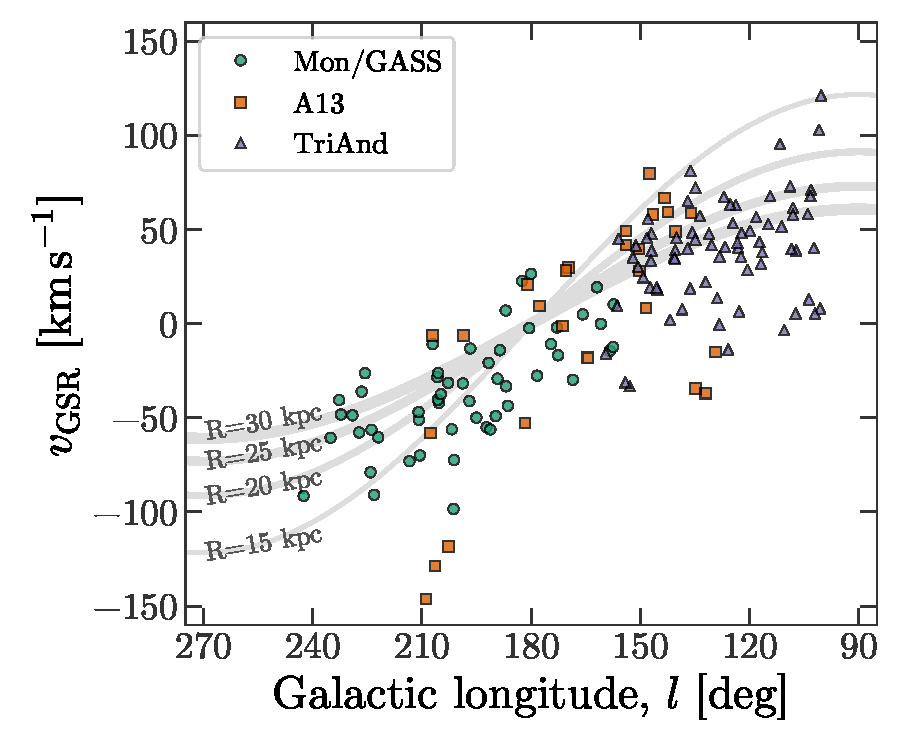
\includegraphics[width=5 in]{figures/vgsr.pdf}
\caption{\label{fig:ting_vel}
Summary of the velocity distribution of M giants in each of the three
low-latitude structures.
Markers represent individual stars identified as likely members of each of the
three structures discussed in this work (see figure legend).
Grey curves show circular orbits in the Galactic disk midplane with circular
velocity equal to $220~\kms$ at several Galactocentric cylindrical radii, $R$,
as indicated on the figure.
Velocity uncertainties are typically the same as or smaller than the marker
sizes.
}
\end{figure}


Figure~\ref{fig:ting_vel} (reproduced from \cite{li17}), summarizes the line-of-sight (GSR) velocity trends of M giants in each of the three low-latitude structures.
Not only do these groups all have low dispersions relative to the stellar halo
--- which confirms  groups themselves as real --- they also
appear to {\it collectively} exhibit a continuous gradient with Galactic longitude,
$l$.
This latter finding suggests that the groups may also be associated with each other.

%{\it Summary: the low latitude structures each have low velocity dispersions supporting the genuine association of the stars within them; they also form velocity sequences as functions of Galactic longitude that are continuous across the groups.}

\subsection{Stellar Populations}
 \label{sec:populations}
Motivated by the observed, low-dispersion velocity distribution of the M giant stars in TriAnd, we sought to observe other distance tracer stars --- RR Lyrae-type pulsators --- in the region, determine their membership, and improve the distance estimates to the structure.
We selected RR Lyrae stars in the TriAnd region from the pre-classified
variable star catalog produced by the Catalina Sky Survey \cite{drake14},
using a conservative distance cut to account for uncertainties in the RR Lyrae
and M giant photometric distance estimates.
We obtained spectra for $\approx$1/3 of the total number of RR Lyrae in the M
giant volume considered to be associated with TriAnd 1 and measured radial
velocities for these stars \cite{pricewhelan15}.

\begin{figure}[t]
\centering
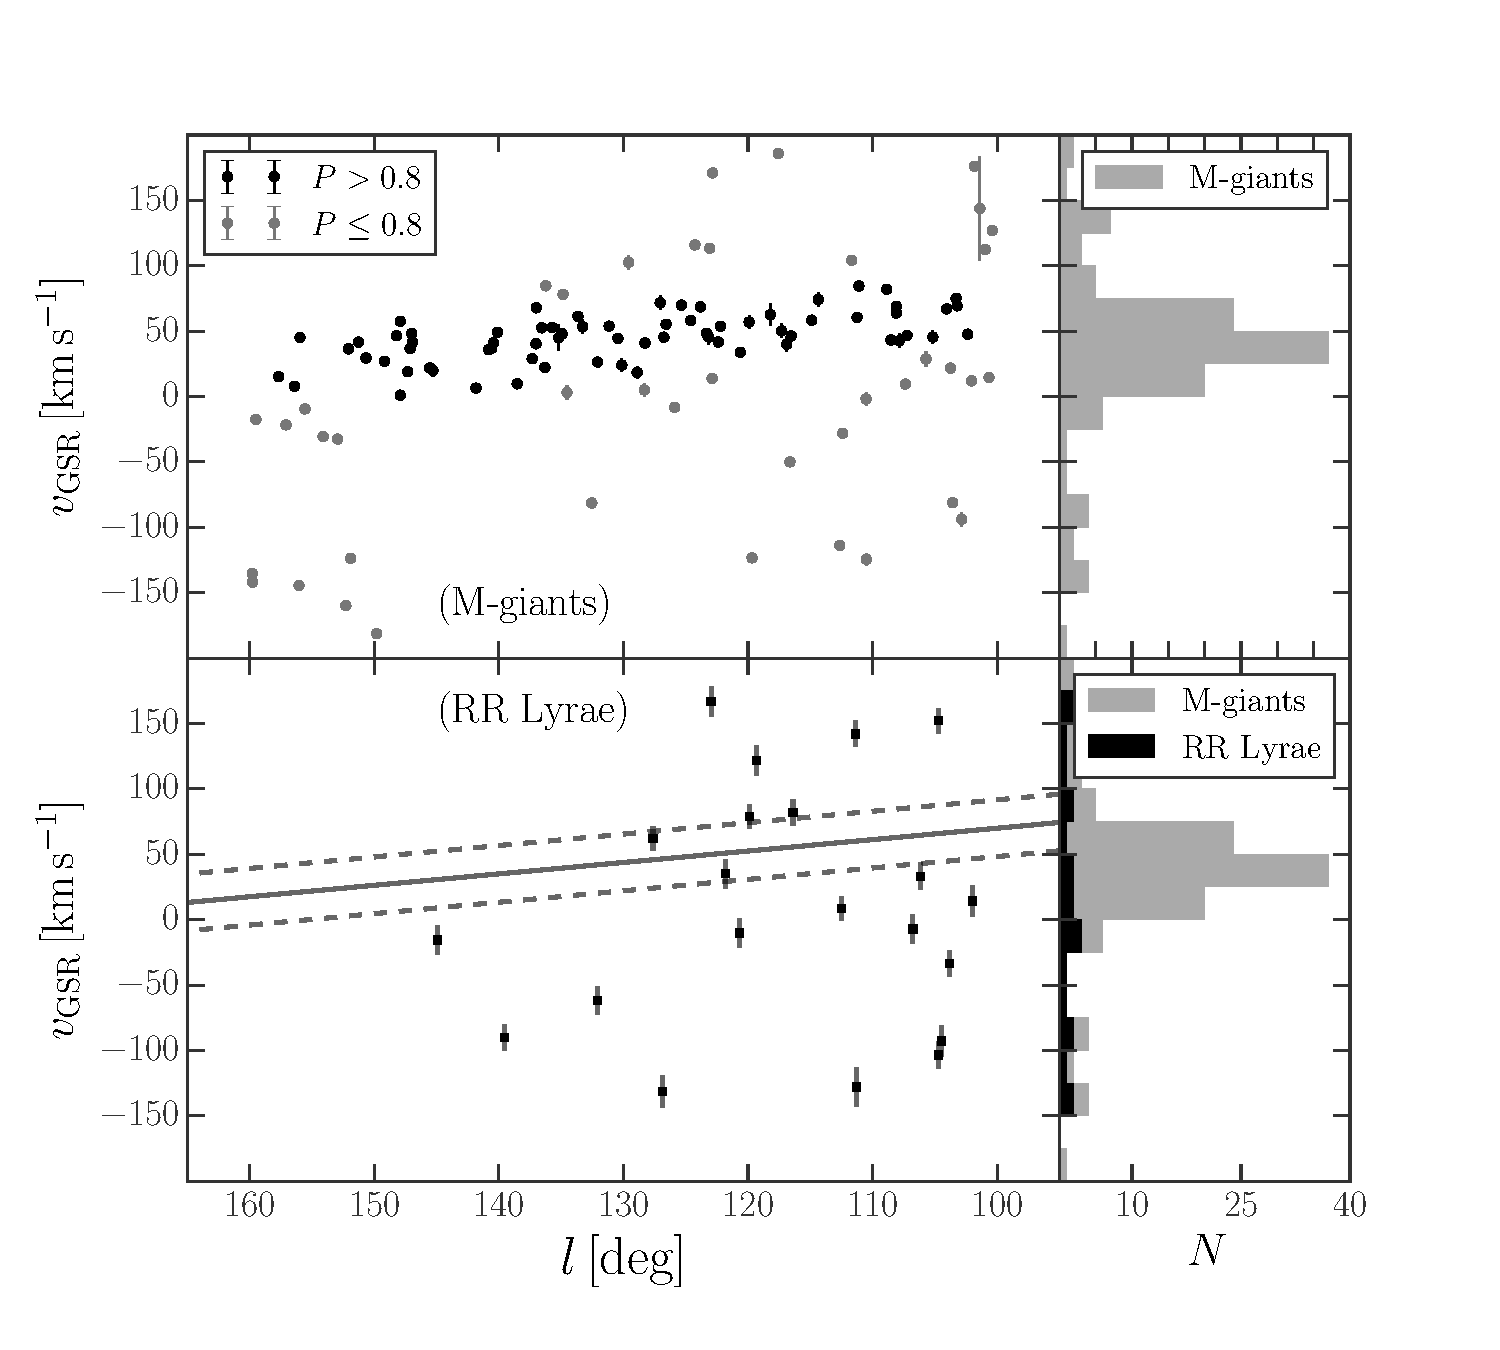
\includegraphics[width=5 in]{figures/triand_rrlyrae}
\caption{\label{fig:apw}
Comparison of the velocity distribution for M giants in the TriAnd structure
(top panel) with velocities for RR Lyrae stars in the same region of sky and
distance range (bottom panel).
}
\end{figure}

Figure~\ref{fig:apw} \cite[reproduced from][]{pricewhelan15} shows the results of our survey: unlike the M giants (gray points) the RR Lyrae (black points) show no clear, tight velocity sequence.
By modeling both the RR Lyrae and M giants velocity data as mixtures of two gaussians representing a cold foreground sequence and a possible background halo population of larger dispersion, we were able to show that the number ratio of RR Lyrae to M giants (\frrmg) within the overdensity was $<0.38$ with 95\% confidence.


%\begin{figure}[t]
%\centering
%
\includegraphics[width=3 cm]{logo-mdpi}
%\caption{\label{fig:isochrones}
%Isochrones for various ages metallicities}
%\end{figure}

Since we were unable to find any RR Lyrae clearly associated with TriAnd 1, our attempt to measure a more accurate distance to this structure was a failure.
However, the upper limit on the value of $\frrmg$ was in itself interesting.
RR Lyrae and M giants are tracers of populations with quite distinct metallicities: stars in the horizontal branch phase of evolution are typically only blue enough to cross the instability strip and become RR Lyrae if they have [Fe/H]$\lesssim -1.5$; and giant stars typically only evolve to colors red enough to become spectral class M if they have [Fe/H]$\gtrsim$-1.5.
Hence, a stellar population has to contain a significant range of metallicities in order to contain both types of stars.
%In order to aid with the interpretation of this discovery, Figure~\ref{fig:isochrones} plots isochrones for two $10~{\rm Gyr}$-old populations of low and intermediate metallicity, including the color range for RR Lyrae and M spectral class.
%It emphasizes our understanding that these two types of stars are tracers of populations with quite distinct metallicities and illustrates why, while the initial aim of our survey to find more accurate distances to TriAnd 1 and 2 had failed, our results could be even more intriguing.
The metallicity distributions in nearly all existing satellite galaxies
orbiting the Milky Way \cite[e.g.,][]{kirby11} are typically biased towards
low metallicities, such that they contain no or few M giant stars (i.e. $\frrmg = \infty$).
The largest satellites (the Large Magellanic Cloud and the Sagittarius dwarf galaxy) are exceptions as they contain the most metal rich populations; these dwarfs have $\frrmg \sim 0.5$ \cite{pricewhelan15}.
In contrast, the Galactic disk is an overall metal-rich population and thus has very few RR Lyrae \cite[i.e. $f_{\rm RR:M} \sim 0$][]{amrose01}, more consistent with our findings for the stellar population of TriAnd 1.

Our work on the stellar populations of the TriAnd region motivated us to look at possible associations of RR Lyrae with the M giant sequences found in Mon/GASS and A13.
For the surveyed regions of these structures, we find \frrmg\ values similar to those observed for TriAnd , and consistent with membership of the Galactic disk. A paper on our results is now in preparation (Sheffield et al 2017).

%{\it Summary: the stellar populations in these groups look like each other; they are more consistent with those in the Galactic disk rather than those observed in the stellar halo or Galactic  satellites.}

\subsection{Abundance Patterns}

\label{sec:abundances}
% APW COMMENT: This section needs more context and perhaps much less detail
% about the actual observations...

The origin of stellar associations can also be explored through the chemical compositions of their constituent stars.
However, our finding (described in Section \ref{sec:populations}) that the low-latitude-structures all have stellar populations (as indicated by $f_{\rm RR:M}$) that look more like the disk than known Galactic satellites is at odds with prior work on abundance patterns.
For example, high-resolution spectra of 21 M giants in Mon/GASS \cite{chou2010b} showed
[Ti/Fe] lower by up to 0.4 dex compared to the mean trends known for main-sequence stars of the Galactic disk (e.g., Reddy et al. 2003, Bensby et al. 2014) and a mean offset for [Y/Fe] of about 0.2 dex at ${\rm [Fe/H]} \approx -0.5$. A comparison with results from the same group for stars in the Sgr dwarf spheroidal galaxy \cite{chou2010a} suggested more similar patterns to those seen in Mon/GASS and support  an external origin for this structure. Subsequent work comes to similar conclusions for the TriAnd Clouds \cite{chou11}.
% APW COMMENT: there are hand-typed references in the paragraph above! We need to add to the bibliography

%It should be noted, however, that their results do not agree with the abundances of Ti and, in particular, La, measured in the Canis Major overdensity by \cite{sbordone2005}. Their analysis was based on spectra covering a limited spectral region in the near-IR, including 11 neutral iron and 2 neutral titanium lines. Also \cite{chou2010b} caution that the effects of non-local thermodynamic equilibrium (non-LTE) may be significant, since their measurement of metallicity and Ti abundances relies on the LTE analysis of lines of neutral species,

In order to explore the apparent contradiction between the stellar populations and abundance work we have recently obtained high-resolution and signal-to-noise spectra of 15 stars in TriAnd 1 and A13 overdensities. 14 stars were observed with the HIRES-S spectrograph at the Keck-1 telescope \cite{vogt1994} and 1 star was observed using the the UVES spectrograph at the VLT (Program ID: 097.B-0770A).
%The spectral resolving power R of the HIRES spectra is 36\,000 and the UVES data have R $\sim$ 47\,000. All Keck spectra cover the full optical region, from $4800$ to $8770$ $\AA$, although the exact wavelength coverage varies as several slightly different instrument configurations were tried in an effort to get all the key lines into a single exposure. The signal-to-noise (SNR)/\AA of the HIRES spectra near 5200 \AA in the continuum at the center of the echelle order exceeds 200. For the UVES spectrum, the SNR of 50 near 5500 \AA was achieved. The fundamental parameters and chemical abundances of stars were determined using 2MASS and APASS photometry and the high-resolution spectra. All 15 stars are M-type giants with effective temperatures Teff ~ 3800 K and surface gravities log(g) ~ 1 dex. The $T_{\rm eff}$ estimates were derived using the Infrared Flux Method (Casagrande et al. 2010, 2014). Chemical abundances were measured for 6 chemical elements, including O, Na, Mg, Ca, Fe, Eu using LTE and the standard MARCS stellar model atmospheres (Gustafsson et al. 2008). We have also performed detailed analysis of the effects of non-local thermodynamic equilibrium (non-LTE) for the elements, where detailed calculations are available \cite{bergemann2011, bergemann2012, bergemann2016}, however, the NLTE corrections for the chosen lines are minor and do not change our conclusions. In what follows, we use our LTE results, because all studies of chemical abundances in dSph systems and most studies in the Milky Way to date have employed LTE with 1D hydrostatic models
We find that stars in the TriAnd 1 and in A13 overdensities have extremely similar chemical abundances, with the abundance dispersion $\leq 0.06$ dex for most chemical elements. The TriAnd 1 and A13 stars also have a very narrow metallicity spread,  ${\rm [Fe/H]} = -0.92 \pm 0.06$ dex. The abundances of all measured alpha-elements are uniformly enhanced at the level of 0.43 $\sim$ 0.06 dex for [O/Fe], 0.41 $\sim$ 0.02 dex for [Mg/Fe], $0.35 \pm 0.06$ dex for [Na/Fe], and 0.15 $\sim$ 0.03 dex for [Eu/Fe]. At this level, the TriAnd 1 and A13 stars are consistent with the abundances of the in-situ formed Milky Way thick disk stars \cite{fuhrmann2004,bergemann2014,bensby2014}.
\footnote{The only exception is [Ca/Fe], which is consistent with solar with the dispersion of 0.06 dex; however, the NLTE abundance correction for the \ion{Ca}{i} lines for M giants is 0.1 dex that will bring the results in agreement with the MW disk studies that are based on FGK dwarfs, for which the NLTE correction is much smaller \cite{Merle2011}}.
The abundance ratios are too high for the chemical abundance patterns observed in the stars of the Galactic satellites (Bonifacio et al. 2010, Shetrone et al. 2001, 2003, Tolstoy et al. 2009, de Boer et al. 2014), which are known to have low, typically solar ( [O/Fe], [Mg/Fe]) or even sub-solar ([Na/Fe]), ratios at [Fe/H] $\sim -1$.
% APW COMMENT: there are hand-typed references in the paragraph above! We need to add to the bibliography

%For example, Fornax, a dSph galaxy most close to TriAnd 1 and A13 in metallicity, has [Na/Fe] $\sim -0.6$ dex and [Mg/Fe] $\sim 0$ at [Fe/H] $=-1$ (Letarte et al. 2010, Kirby 2010, Lemasle et al. 2014) \footnote{Note that to avoid systematic differences between abundance measurements obtained from spectra taken with different instruments, we have chosen here to compare with the data taken with the same instrument; here UVES and FLAMES at the VLT, ESO, or with HIRES at Keck.}.

%Our results for TriAnd and A13 do not confirm the conclusions by \cite{chou2010b}. Although there could be several astrophysical reasons for the differences, this could be caused by the
One explanation for the disagreement between abundance work for stars in the same structure is
differences in the observed datasets and spectroscopic modeling techniques.
%Our observed data cover the full optical range from the near-UV to the near-IR, whereas
\cite{chou2010b} analysed a small wavelength region in the near-IR, limited to 150 \AA from 7440 to 7590 \AA. Because of this limitation, they could include only 11 \ion{Fe}{I} and 2 \ion{Ti}{I} lines in the determination of gravities, metallicities, and abundances. Our analysis, through a much wider wavelength coverage and high SNR attained for the observed spectra, allowed us to include 70 lines of \ion{Fe}{I} and \ion{Fe}{II} \cite{bergemann2012}, as well as 10 lines of \ion{Ti}{2}. Moreover,  \cite{bergemann2011} showed that \ion{Ti}{1} should be not be used in abundance studies because it is very sensitive to NLTE effects .
In order to explore the the sensitivity of abundance diagnostics to the line selection and wavelength regimes we performed test computations on our own data, using a reduced linelist. We have found that using the linelist from \cite{chou2010a}, the metallicities are over-estimated by $\sim 0.25$ dex and [Ti/Fe] are under-estimated by $0.4$ dex, compared to the results using the complete linelist. This suggests that the choice of the linelist and diagnostic spectral band (full optical or near-IR) as a plausible explanation  of the apparently discrepant results.
%{\it Summary: the abundance patterns  of the low-latitude structures are similar to those of the thick disk of our Galaxy.}

Overall, comparing our work to abundances of disk stars and satellite populations obtained using analogous data sets and reduction techniques, our results suggest that the birthplace of stars in TriAnd 1 and A13 was the outer Galactic disk rather than an infalling satellite galaxy.
A paper describing this work is currently in preparation (Bergemann et al., in prep.).

% APW COMMENT: there are hand-typed references in the paragraph above! We need to add to the bibliography

%it is unlikely that the TriAnd 1 and A13 stars originate from a disrupted dSph galaxy

\subsection{Photometric Surveys}

% APW COMMENT: If the sections are reorganized to be by structure instead, this
% should be moved to the section on Mon/GASS, I believe
While we have concentrated on follow-up studies of the known low-latitude structures as traced by M giants selected from 2MASS, knowledge of the spatial distribution of stars towards the anticenter region has been further refined using photometry in SDSS \cite{xu15} and PanSTARRS \cite{kaiser10,lurie17}.
Both these studies employed the novel technique of subtracting color-magnitude diagrams (CMD's) derived from fields in their photometric data which were symmetrically placed at equal and opposite Galactic latitudes and at the same Galactic longitudes.
These differenced CMD's allowed denser regions, closer to the Galactic plane and at smaller heliocentric distances  to be explored.
Both studies showed overdense arcs or stars oscillating between the northern and southern hemispheres as the distance from the Sun was increased towards the anticenter of our Galaxy.
The vast numbers of stars in these surveys allowed more clear identification of these global structures as clearly distinct, separate features.

%{\it Summary: the overdensities around the outer Galaxy, oscillating between the northern and southern hemispheres have been traced to smaller-scale oscillations all the way to the Solar Neighborhood.}



% APW COMMENT: If you reorganize, I would move the discussion of simulations of
% individual structures to their respective sections about. Instead, I would
% make this section something like "Theoretical interpretations of the global
% structure of the outer disk"

\subsection{Local Spectroscopic Surveys}

% APW COMMENT: If the sections are reorganized to be by structure instead,
% this could get moved to the discussion. "Discussion: connections to velocity
% structure near the Sun" or something

Coincident with these studies exploring structures at the very outer edge of our Galactic disk,
large scale spectroscopic surveys have allowed a detailed re-examination of the {\it local} distribution of stellar velocities.
Asymmetries between the Northern and Southern Galactic hemispheres in the vicinity of the Sun have been seen in the density and velocity distributions using data from SDSS \cite{widrow12,yanny13} and RAdial Velocity Experiment \cite[RAVE, see][]{??,williams13}.
Looking $\sim$2kpc out towards the Galactic anticenter, the Large Sky Area Multi-Object Fiber Spectroscopic Telescope \cite[LAMOST,][]{cui12,deng12,zhao12} finds similar asymmetries in radial and vertical velocities \cite{carlin13}.
The scale and sense of these asymmetries indicate moderate systematic motions (of order a few km/s)  of stars within the disk perpendicular to the plane,  suggesting both vertical movement of midplane, and compression and rarefaction of the vertical scale \cite[referred to as ``bending'' and ``breathing'' modes respectively --- see,][]{widrow14}.
It is natural to associate these asymmetries in motion as a local manifestations of the oscillations traced in space over much larger scales \cite{xu15,pricewhelan15}.
%{\it Summary: small-scale, systematic vertical motions of and within the disk have been detected in the Solar Neighborhood.}


\section{The Nature of Structures Around the Outer Disk --- Summary of Theoretical Interpretations}
\label{sec:theory}

The observations summarized in Section \ref{sec:obs} indicate that:
\begin{itemize}
\item the low latitude structures --- Mon/GASS, TriAnd 1/2 and A13  --- each have low velocity dispersions supporting the genuine association of the stars within them;
\item Mon/GASS, TriAnd 1/2 and A13 also share a single, continuous sequence in average velocity as a function of $l$ suggestive of associations across these groups;
\item the stellar populations (as indicated by $f_{\rm RR:M}$) in these groups look like each other;
\item the stellar populations are more consistent with those in the Galactic disk rather than those observed in the stellar halo or Galactic  satellites;
\item the abundance patterns  of the low-latitude structures are similar to those of the thick disk of our Galaxy;
\item the low-latitude structures around the outer Galaxy can be connected to overdensities oscillating between the northern and southern hemispheres on smaller scales and traced all the way back to the Solar Neighborhood;
\item small-scale, systematic vertical motions of and within the disk have been detected in the Solar Neighborhood which suggest the local disk is moving up and down.
\end{itemize}

\begin{figure}[t]
\centering
\includegraphics[width=4 in]{figures/cartoon.pdf}
\caption{\label{fig:cartoon}
TODO: Cartoon of oscillations in space and velocity}
\end{figure}

Figure \ref{fig:cartoon} is a cartoon which summarizes all the observational works and their implications, by showing the approximate locations and amplitudes of the spatial and velocity structures that have been identified. (Note that the figure is misleading as the structures are {\it not} consistent morphologically with concentric rings that are axisymmetric about the Galactic center.)
Taken together, we conclude that: (i) there is compelling evidence that Mon/GASS, TriAnd 1/2 and A13 represent populations of stars formed in the disk that now exist at extreme $(R,Z)$;
(ii) these structures are associated with each other as part of a global system of vertical disk oscillations that can be traced all the way to the velocity asymmetries seen in the Solar Neighborhood; and
(iii) the stellar populations in these structures are inconsistent with a picture where they formed from an accreted satellite.

One natural interpretation of these collected observations is that the oscillations represent the response of the disk to an external perturbation, for example as the impact of a satellite galaxy is transmitted and amplified by its wake in the dark matter halo \cite[as described for the LMC in][]{weinberg06}
Prior work has already pointed to this as a possible explanation for the existence of Mon/GASS \cite{kazantzidis08,younger08}, with the Sagittarius dwarf galaxy being pointed to as a plausible culprit for the perturbation \cite{purcell11}.
It has also been demonstrated how perturbations from a satellite on an orbit perpendicular to the disk could lead to bending (at low relative impact velocity) and breathing (at higher relative velocity) modes that would be observed in the Solar Neighborhood as asymmetries in the local velocity distribution  \cite{widrow14} and on larger scales as rings \cite{donghia16}.
Simulations have also shown that Sgr could be responsible for local velocity structure  \cite{gomez13}.
Such interactions and corresponding disk features have been found to naturally occur in cosmological simulations \cite{gomez16}.

\begin{figure}[t]
\centering
%
\includegraphics[width=3 cm]{logo-mdpi}
\caption{\label{fig:chervin}
}
\end{figure}

Figure \ref{fig:chervin} illustrates these ideas with the results of simulations from our own recent work.
We extended the prior theoretical backdrop that looked at Mon/GASS to examine whether the extreme locations of TriAnd 1/2 could fit within the same picture using simulations of a disk disturbed (separately) by satellites on orbits that mimic those expected for the Large Magellanic Cloud and Sagittarius \cite{laporte16}.
With different masses and orbits (and consequently different interaction  strength, timings, and durartions) these satellite necessarily induced distinct but overlapping signatures.
In  more recent work, we found that a model that was capable of reproducing the scales of the observed disturbances (radial wavelength and  amplitude in space, as well as magnitude of offsets in velocity locally) needed:
the  interaction of Sgr with the disk of the Milky Way to be followed for several passages longer than prior work;
Sgr to have of sufficient initial mass and density to impact the disk in the last Gigayear with a remaining mass of ???;
and the disk to be realized with stars existing as far out as ???kpc form the Galactic center in order to populate the regions corresponding to TriAnd 1/2.
The interaction with the LMC modified the overall morphology of the structures induced, but was not sufficient alone to explain their properties.
The full details of these results will be discussed in an upcoming paper (Laporte et al, 2017).

\section{Discussion --- Observational Prospects}

\subsection{The Milky Way}

%It is interesting to place the current work in the context of ongoing and near-future studies of our Galaxy.
While the connections that have already been made between the different low-latitude structures and of these structures with the disk population are convincing, there are several directions for further observations which would greatly facilitate an informative comparison to theoretical work, allowing more detailed interpretations and tighter constraints on matter distributions and histories.

The most obvious first direction would be to increase the dimensions of motion and accuracy of distance estimates to known features.
For example,  proper motions for the ``Anti-Center Stream'' (ACS) \cite[which may or may not be part of the larger Mon/GASS structure, see ] []{li12} indicate that stars in the ACS are not actually moving parallel to the stream \cite{carlin10}. This is inconsistent with expectations for the behavior of debris from a destroyed satellite.
If similar measurements of proper motions of stars in all the low-latitude structures showed significant motion perpendicular to the Galactic disk, this would provide the final evidence of a disk origin and connection to local oscillations, as well as important constraints on dynamical models (see Section \ref{sec:conc}).
In near-future data-releases, ESA's {\it Gaia} satellite \cite{???} is poised to provide just such proper motion data --- with proper motion accuracies of ??? $\mu$as/year or ?? km/s for our (closest) ??? mag M giant stars in Mon/GASS and ??? $\mu$as/year or ?? km/s for our (farthest) ??? mag M giant stars in TriAnd.

The second direction is to extend the various maps to to fainter magnitudes and global scales. Again, {\it Gaia} will be able to tackle this with distances, proper motions and radial velocities, although its reach towards low latitudes in the inner Galaxy will be limited by extinction.
Infrared surveys, such as APOGEE \cite{apogee}, could overcome this limitation and reach entirely across the Galaxy. Spectra from such a survey could provide both motions and abundance patterns.

\subsection{Other Galaxies}

The great advantage of star-count studies is the ability to reach extremely low surface brightness levels. For example, the TriAnd clouds have been estimated to have surface brightness lower than
$\Sigma <$32 mag/arcsec$^2$ \cite{majewski04}.
%For example, TriAnd I contains ?? M-giant stars spread over an area on the sky of roughly ????, so ? giants/deg$^2$.
%Adopting a 10 Gyr-old isochrone for this population \cite[from the Padova group][]{}, each M-giant has an associated total stellar luminosity of ??? in the ?? band. Hence, the equivalanet urfc ebright ness would be .....

The growing samples of galaxies within and beyond the Local Group being mapped to extremely low surface brightness levels are intriguing.
Nearby, these can be reached, like the Milky Way, through star counts studies, most spectacularly for the case of our nearest neighbor, the Andromeda Galaxy, where giant star counts have revealed a significantly extended and richly featured outer stellar disk \cite{ferguson02,ibata05}.
Analogous studies have been carried out for galaxies up to distances of several Mpc \cite[e.g.,][]{monachesi13,crnojevi16}, although the focus of these studies has typically been on detecting the stellar halo of these objects.
Several dedicated surveys have made innovative advances in studying galaxies to LSB using a variety of techniques to reach limits below 30  mag/arcsec$^2$ in integrated light \citep[e.g.][]{delgado10,vandokkum14,duc15}.

Looking to the future,
NASA's proposed WFIRST satellite, with its wide field of view and high resolution, offers the possibility of extending the deep star-count sensitivities now achieved in MW and M31 to all galaxies within 10 Mpc \cite{spergel13}; and
the next decade will also see first light for the Large Synoptic Survey Telescope (LSST), from which images can be combined to be sensitive to slightly shallower depth \citep[$\sim$29 mag/arcsec$^2$, see][]{ivezic08} but for vast numbers (many millions!) of galaxies.


\section{Conclusion --- What Might These Structures Tell Us About Galaxies?}

%{\it KVJ --- Reminder to self to add these somewhere} \\
%arXiv:1706.01900  --- Title: Milky Way Tomography with K and M Dwarf Stars: the Vertical Structure of the Galactic Disk \\
 %D'Onghia et al 2016 on sat and disk interaction \\
% Bovy et al 2015 - power spectrum of vel in disk \\
% Kazantzidis08 - rings etc \\
% schwarzkopf 01 \\
 %Zarik=tsky 97 - lopsided gals and accreiton

\label{sec:conc}

The above sections  summarized observational evidence for large scale vertical oscillations of the Galactic plane present in the Solar Neighborhood and reaching out beyond the traditional edge of our stellar disk.
They also collated theoretical studies that suggest that these oscillations could be caused by, and contain the signatures of, ongoing interactions of the Milky Way with its satellite system.
Moreover, observational prospects are bright for extending this work both to globally map the Milky Way, and to look for analogous features around many other galaxies.

Now that we have a physical picture of the origin of such features, as well as prospects for mapping them further within the Milky Way and detecting analogous substructures around other galaxies, we can move on to discussing how useful they are as probes of dynamics and history.
It is important to have these uses in mind to motivate and frame  future work.
While the mere existence of these structures is interesting, they contain a tiny fraction of the stars in galaxies spread out over a large area --- these properties naturally make them difficult to map, either because their unique signatures can be lost in the foreground star counts (e.g., in the Milky Way), or  because the required surface brightness limits for detection are prohibitively low (for integrated light).

Conversely, these features around the outskirts of galaxies may prove to be particularly powerful probes of interactions and histories, precisely because they contain so little mass --- they can be modeled rather simply as test particles responding to an external perturbation.

Below are just three examples of where these structures could promise new insights into some classic questions.
\begin{description}
\item{\it Disk heating mechanisms ---}
It has been understood for a long time that disks can evolve significantly due to mergers, major or minor, and hence that their current structures bear witness to their accretion history \cite{toth92,quinn93,walker96,velazquez99}.
This understanding has fueled a significant literature on the importance of the heating of galactic disks in response to encounters with other dark matter halos (that may or may not contain their own galaxies) \cite{font01,ardi03,benson04,stewart08,hopkins08,villalobos08,purcell09,kazantzidis09,sachdeva16,moetazedian16}.
In general, these studies have concentrated on the overall effects of many encounters on global properties, such as the thickness and vertical velocity dispersion in disks.
Their results have traditionally been compared to these scales in samples of galaxies.
In contrast, the identification and mapping of vertical waves in our Milky Way associated with ongoing interactions gives us the opportunity to dissect an individual disk heating event in progress.
We can use this to check our understanding of the mechanism directly and in detail rather than assessing its importance through collective effects and longterm, phase-mixed signatures.
\item{\it Stellar halo formation processes ----}
The last decade has seen increasing interest in assessing how much of the content of stellar halos could be made from stars originally formed in the disks of the galaxies that they surround. Hydrodynamical simulations of galaxy formaion suggest that tens of percent of the inner halo might be formed this way
\cite{abadi06,zolotov09,zolotov10,font11,mccarthy12,tissera13,tissera14,pillepich15,cooper15}.
Preliminary arguments for the existence of this ``kicked-out-disk'' population were based on transitions in the density or orbital structures of stellar halos \cite[e.g.,][]{carollo07}.
However, such transitions were also found to naturally occur in purely-accreted models of stellar halos \cite{deason13}.
More convincing observational evidence for disk stars in the halo is just beginning to emerge through studies with look for stars with halo-like kinematics, but disk-like abundances around M31 \cite{dorman13} and the Milky Way \cite{sheffield12,hawkins15,bonaca17}.
Our own work adds new perspectives on this stellar halo formation process with the detection and modeling of disk stars that may be in transition from the disk to the halo.
\item{\it Galactoseismic probes of interactions and dark matter ---}
The response of a disk to an encounter will depend on its own properties, the properties of the dark matter halo in which it is embedded and the mass and orbit of the perturbing satellite.
This leads to the suggestion that, analogous to helioseismic investigations of the structure of our Sun, maps of a disk response --- such as those described in Section \ref{sec:obs} for our Milky Way --- might be similarly inverted to tell us about (e.g.) the structure of the dark matter halo
\cite{widrow12}.
Indeed, recent studies of the signatures of encounters in the very outskirts of extended HI disks have successfully used simulations combined with an analytic understanding to find how the observed characteristics of the disturbed gas can be simply related to properties of the perturbing object \cite{chakrabarti09,chakrabarti11b,chang11}.
\end{description}

Uplifting/Concluding sentence.

%%%%%%%%%%%%%%%%%%%%%%%%%%%%%%%%%%%%%%%%%%
\vspace{6pt}

%%%%%%%%%%%%%%%%%%%%%%%%%%%%%%%%%%%%%%%%%%
%% optional
%\supplementary{The following are available online at www.mdpi.com/link, Figure S1: title, Table S1: title, Video S1: title.}

%%%%%%%%%%%%%%%%%%%%%%%%%%%%%%%%%%%%%%%%%%
\acknowledgments{Much of the work reviewed in this paper was made possible by NSF grants AST-1312196.
K.V.J. was supported by NSF grant AST-1614743 while writing the review.}

%%%%%%%%%%%%%%%%%%%%%%%%%%%%%%%%%%%%%%%%%%
\authorcontributions{This paper summarizes results from the team of listed authors. It was written by K.V.J and A.P.W., with section contributions from M.B.. Figures were made by Adrian Price-Whelan and C.L.. All the authors reviewed and commented on the drafts.}

%%%%%%%%%%%%%%%%%%%%%%%%%%%%%%%%%%%%%%%%%%
\conflictsofinterest{The authors declare no conflict of interest.}

%%%%%%%%%%%%%%%%%%%%%%%%%%%%%%%%%%%%%%%%%%
%% optional
%\abbreviations{The following abbreviations are used in this manuscript:\\

%\noindent
%\begin{tabular}{@{}ll}
%MDPI & Multidisciplinary Digital Publishing Institute\\
%DOAJ & Directory of open access journals\\
%TLA & Three letter acronym\\
%LD & linear dichroism
%\end{tabular}}

%%%%%%%%%%%%%%%%%%%%%%%%%%%%%%%%%%%%%%%%%%
%%%%%%%%%%%%%%%%%%%%%%%%%%%%%%%%%%%%%%%%%%
% Citations and References in Supplementary files are permitted provided that they also appear in the reference list here.

%=====================================
% References, variant A: internal bibliography
%=====================================
\externalbibliography{yes}
% \bibliographystyle{chicago2}
\bibliography{refs}

% \begin{thebibliography}{-------}
%\providecommand{Natureexlab}[1]{#1}

\bibitem[{ESA}(1997)]{esa97}
{ESA}., Ed.
\newblock {\em {The HIPPARCOS and TYCHO catalogues. Astrometric and photometric
  star catalogues derived from the ESA HIPPARCOS Space Astrometry Mission}},
  Vol. 1200, {\em ESA Special Publication},  1997.

\bibitem[{Dehnen}(1998)]{dehnen98}
{Dehnen}, W.
\newblock {The Distribution of Nearby Stars in Velocity Space Inferred from
  HIPPARCOS Data}.
\newblock {\em AJ} {\bf 1998}, {\em 115},~2384--2396,
  \href{http://xxx.lanl.gov/abs/astro-ph/9803110}{{\normalfont
  [astro-ph/9803110]}}.

\bibitem[{Dehnen}(2000)]{dehnen00}
{Dehnen}, W.
\newblock {The Effect of the Outer Lindblad Resonance of the Galactic Bar on
  the Local Stellar Velocity Distribution}.
\newblock {\em AJ} {\bf 2000}, {\em 119},~800--812,
  \href{http://xxx.lanl.gov/abs/astro-ph/9911161}{{\normalfont
  [astro-ph/9911161]}}.

\bibitem[{York} \em{et~al.}(2000){York}, {Adelman}, {Anderson}, {Anderson},
  {Annis}, {Bahcall}, {Bakken}, {Barkhouser}, {Bastian}, {Berman}, {Boroski},
  {Bracker}, {Briegel}, {Briggs}, {Brinkmann}, {Brunner}, {Burles}, {Carey},
  {Carr}, {Castander}, {Chen}, {Colestock}, {Connolly}, {Crocker}, {Csabai},
  {Czarapata}, {Davis}, {Doi}, {Dombeck}, {Eisenstein}, {Ellman}, {Elms},
  {Evans}, {Fan}, {Federwitz}, {Fiscelli}, {Friedman}, {Frieman}, {Fukugita},
  {Gillespie}, {Gunn}, {Gurbani}, {de Haas}, {Haldeman}, {Harris}, {Hayes},
  {Heckman}, {Hennessy}, {Hindsley}, {Holm}, {Holmgren}, {Huang}, {Hull},
  {Husby}, {Ichikawa}, {Ichikawa}, {Ivezi{\'c}}, {Kent}, {Kim}, {Kinney},
  {Klaene}, {Kleinman}, {Kleinman}, {Knapp}, {Korienek}, {Kron}, {Kunszt},
  {Lamb}, {Lee}, {Leger}, {Limmongkol}, {Lindenmeyer}, {Long}, {Loomis},
  {Loveday}, {Lucinio}, {Lupton}, {MacKinnon}, {Mannery}, {Mantsch}, {Margon},
  {McGehee}, {McKay}, {Meiksin}, {Merelli}, {Monet}, {Munn}, {Narayanan},
  {Nash}, {Neilsen}, {Neswold}, {Newberg}, {Nichol}, {Nicinski}, {Nonino},
  {Okada}, {Okamura}, {Ostriker}, {Owen}, {Pauls}, {Peoples}, {Peterson},
  {Petravick}, {Pier}, {Pope}, {Pordes}, {Prosapio}, {Rechenmacher}, {Quinn},
  {Richards}, {Richmond}, {Rivetta}, {Rockosi}, {Ruthmansdorfer}, {Sandford},
  {Schlegel}, {Schneider}, {Sekiguchi}, {Sergey}, {Shimasaku}, {Siegmund},
  {Smee}, {Smith}, {Snedden}, {Stone}, {Stoughton}, {Strauss}, {Stubbs},
  {SubbaRao}, {Szalay}, {Szapudi}, {Szokoly}, {Thakar}, {Tremonti}, {Tucker},
  {Uomoto}, {Vanden Berk}, {Vogeley}, {Waddell}, {Wang}, {Watanabe},
  {Weinberg}, {Yanny}, {Yasuda}, and {SDSS Collaboration}]{york00}
{York}, D.G.; {Adelman}, J.; {Anderson}, Jr., J.E.; {Anderson}, S.F.; {Annis},
  J.; {Bahcall}, N.A.; {Bakken}, J.A.; {Barkhouser}, R.; {Bastian}, S.;
  {Berman}, E.; {Boroski}, W.N.; {Bracker}, S.; {Briegel}, C.; {Briggs}, J.W.;
  {Brinkmann}, J.; {Brunner}, R.; {Burles}, S.; {Carey}, L.; {Carr}, M.A.;
  {Castander}, F.J.; {Chen}, B.; {Colestock}, P.L.; {Connolly}, A.J.;
  {Crocker}, J.H.; {Csabai}, I.; {Czarapata}, P.C.; {Davis}, J.E.; {Doi}, M.;
  {Dombeck}, T.; {Eisenstein}, D.; {Ellman}, N.; {Elms}, B.R.; {Evans}, M.L.;
  {Fan}, X.; {Federwitz}, G.R.; {Fiscelli}, L.; {Friedman}, S.; {Frieman},
  J.A.; {Fukugita}, M.; {Gillespie}, B.; {Gunn}, J.E.; {Gurbani}, V.K.; {de
  Haas}, E.; {Haldeman}, M.; {Harris}, F.H.; {Hayes}, J.; {Heckman}, T.M.;
  {Hennessy}, G.S.; {Hindsley}, R.B.; {Holm}, S.; {Holmgren}, D.J.; {Huang},
  C.h.; {Hull}, C.; {Husby}, D.; {Ichikawa}, S.I.; {Ichikawa}, T.;
  {Ivezi{\'c}}, {\v Z}.; {Kent}, S.; {Kim}, R.S.J.; {Kinney}, E.; {Klaene}, M.;
  {Kleinman}, A.N.; {Kleinman}, S.; {Knapp}, G.R.; {Korienek}, J.; {Kron},
  R.G.; {Kunszt}, P.Z.; {Lamb}, D.Q.; {Lee}, B.; {Leger}, R.F.; {Limmongkol},
  S.; {Lindenmeyer}, C.; {Long}, D.C.; {Loomis}, C.; {Loveday}, J.; {Lucinio},
  R.; {Lupton}, R.H.; {MacKinnon}, B.; {Mannery}, E.J.; {Mantsch}, P.M.;
  {Margon}, B.; {McGehee}, P.; {McKay}, T.A.; {Meiksin}, A.; {Merelli}, A.;
  {Monet}, D.G.; {Munn}, J.A.; {Narayanan}, V.K.; {Nash}, T.; {Neilsen}, E.;
  {Neswold}, R.; {Newberg}, H.J.; {Nichol}, R.C.; {Nicinski}, T.; {Nonino}, M.;
  {Okada}, N.; {Okamura}, S.; {Ostriker}, J.P.; {Owen}, R.; {Pauls}, A.G.;
  {Peoples}, J.; {Peterson}, R.L.; {Petravick}, D.; {Pier}, J.R.; {Pope}, A.;
  {Pordes}, R.; {Prosapio}, A.; {Rechenmacher}, R.; {Quinn}, T.R.; {Richards},
  G.T.; {Richmond}, M.W.; {Rivetta}, C.H.; {Rockosi}, C.M.; {Ruthmansdorfer},
  K.; {Sandford}, D.; {Schlegel}, D.J.; {Schneider}, D.P.; {Sekiguchi}, M.;
  {Sergey}, G.; {Shimasaku}, K.; {Siegmund}, W.A.; {Smee}, S.; {Smith}, J.A.;
  {Snedden}, S.; {Stone}, R.; {Stoughton}, C.; {Strauss}, M.A.; {Stubbs}, C.;
  {SubbaRao}, M.; {Szalay}, A.S.; {Szapudi}, I.; {Szokoly}, G.P.; {Thakar},
  A.R.; {Tremonti}, C.; {Tucker}, D.L.; {Uomoto}, A.; {Vanden Berk}, D.;
  {Vogeley}, M.S.; {Waddell}, P.; {Wang}, S.i.; {Watanabe}, M.; {Weinberg},
  D.H.; {Yanny}, B.; {Yasuda}, N.; {SDSS Collaboration}.
\newblock {The Sloan Digital Sky Survey: Technical Summary}.
\newblock {\em AJ} {\bf 2000}, {\em 120},~1579--1587,
  \href{http://xxx.lanl.gov/abs/astro-ph/0006396}{{\normalfont
  [astro-ph/0006396]}}.

\bibitem[{Stoughton} \em{et~al.}(2002){Stoughton}, {Lupton}, {Bernardi},
  {Blanton}, {Burles}, {Castander}, {Connolly}, {Eisenstein}, {Frieman},
  {Hennessy}, {Hindsley}, {Ivezi{\'c}}, {Kent}, {Kunszt}, {Lee}, {Meiksin},
  {Munn}, {Newberg}, {Nichol}, {Nicinski}, {Pier}, {Richards}, {Richmond},
  {Schlegel}, {Smith}, {Strauss}, {SubbaRao}, {Szalay}, {Thakar}, {Tucker},
  {Vanden Berk}, {Yanny}, {Adelman}, {Anderson}, {Anderson}, {Annis},
  {Bahcall}, {Bakken}, {Bartelmann}, {Bastian}, {Bauer}, {Berman},
  {B{\"o}hringer}, {Boroski}, {Bracker}, {Briegel}, {Briggs}, {Brinkmann},
  {Brunner}, {Carey}, {Carr}, {Chen}, {Christian}, {Colestock}, {Crocker},
  {Csabai}, {Czarapata}, {Dalcanton}, {Davidsen}, {Davis}, {Dehnen},
  {Dodelson}, {Doi}, {Dombeck}, {Donahue}, {Ellman}, {Elms}, {Evans}, {Eyer},
  {Fan}, {Federwitz}, {Friedman}, {Fukugita}, {Gal}, {Gillespie}, {Glazebrook},
  {Gray}, {Grebel}, {Greenawalt}, {Greene}, {Gunn}, {de Haas}, {Haiman},
  {Haldeman}, {Hall}, {Hamabe}, {Hansen}, {Harris}, {Harris}, {Harvanek},
  {Hawley}, {Hayes}, {Heckman}, {Helmi}, {Henden}, {Hogan}, {Hogg}, {Holmgren},
  {Holtzman}, {Huang}, {Hull}, {Ichikawa}, {Ichikawa}, {Johnston}, {Kauffmann},
  {Kim}, {Kimball}, {Kinney}, {Klaene}, {Kleinman}, {Klypin}, {Knapp},
  {Korienek}, {Krolik}, {Kron}, {Krzesi{\'n}ski}, {Lamb}, {Leger},
  {Limmongkol}, {Lindenmeyer}, {Long}, {Loomis}, {Loveday}, {MacKinnon},
  {Mannery}, {Mantsch}, {Margon}, {McGehee}, {McKay}, {McLean}, {Menou},
  {Merelli}, {Mo}, {Monet}, {Nakamura}, {Narayanan}, {Nash}, {Neilsen},
  {Newman}, {Nitta}, {Odenkirchen}, {Okada}, {Okamura}, {Ostriker}, {Owen},
  {Pauls}, {Peoples}, {Peterson}, {Petravick}, {Pope}, {Pordes}, {Postman},
  {Prosapio}, {Quinn}, {Rechenmacher}, {Rivetta}, {Rix}, {Rockosi}, {Rosner},
  {Ruthmansdorfer}, {Sandford}, {Schneider}, {Scranton}, {Sekiguchi}, {Sergey},
  {Sheth}, {Shimasaku}, {Smee}, {Snedden}, {Stebbins}, {Stubbs}, {Szapudi},
  {Szkody}, {Szokoly}, {Tabachnik}, {Tsvetanov}, {Uomoto}, {Vogeley}, {Voges},
  {Waddell}, {Walterbos}, {Wang}, {Watanabe}, {Weinberg}, {White}, {White},
  {Wilhite}, {Wolfe}, {Yasuda}, {York}, {Zehavi}, and {Zheng}]{stoughton02}
{Stoughton}, C.; {Lupton}, R.H.; {Bernardi}, M.; {Blanton}, M.R.; {Burles}, S.;
  {Castander}, F.J.; {Connolly}, A.J.; {Eisenstein}, D.J.; {Frieman}, J.A.;
  {Hennessy}, G.S.; {Hindsley}, R.B.; {Ivezi{\'c}}, {\v Z}.; {Kent}, S.;
  {Kunszt}, P.Z.; {Lee}, B.C.; {Meiksin}, A.; {Munn}, J.A.; {Newberg}, H.J.;
  {Nichol}, R.C.; {Nicinski}, T.; {Pier}, J.R.; {Richards}, G.T.; {Richmond},
  M.W.; {Schlegel}, D.J.; {Smith}, J.A.; {Strauss}, M.A.; {SubbaRao}, M.;
  {Szalay}, A.S.; {Thakar}, A.R.; {Tucker}, D.L.; {Vanden Berk}, D.E.; {Yanny},
  B.; {Adelman}, J.K.; {Anderson}, Jr., J.E.; {Anderson}, S.F.; {Annis}, J.;
  {Bahcall}, N.A.; {Bakken}, J.A.; {Bartelmann}, M.; {Bastian}, S.; {Bauer},
  A.; {Berman}, E.; {B{\"o}hringer}, H.; {Boroski}, W.N.; {Bracker}, S.;
  {Briegel}, C.; {Briggs}, J.W.; {Brinkmann}, J.; {Brunner}, R.; {Carey}, L.;
  {Carr}, M.A.; {Chen}, B.; {Christian}, D.; {Colestock}, P.L.; {Crocker},
  J.H.; {Csabai}, I.; {Czarapata}, P.C.; {Dalcanton}, J.; {Davidsen}, A.F.;
  {Davis}, J.E.; {Dehnen}, W.; {Dodelson}, S.; {Doi}, M.; {Dombeck}, T.;
  {Donahue}, M.; {Ellman}, N.; {Elms}, B.R.; {Evans}, M.L.; {Eyer}, L.; {Fan},
  X.; {Federwitz}, G.R.; {Friedman}, S.; {Fukugita}, M.; {Gal}, R.;
  {Gillespie}, B.; {Glazebrook}, K.; {Gray}, J.; {Grebel}, E.K.; {Greenawalt},
  B.; {Greene}, G.; {Gunn}, J.E.; {de Haas}, E.; {Haiman}, Z.; {Haldeman}, M.;
  {Hall}, P.B.; {Hamabe}, M.; {Hansen}, B.; {Harris}, F.H.; {Harris}, H.;
  {Harvanek}, M.; {Hawley}, S.L.; {Hayes}, J.J.E.; {Heckman}, T.M.; {Helmi},
  A.; {Henden}, A.; {Hogan}, C.J.; {Hogg}, D.W.; {Holmgren}, D.J.; {Holtzman},
  J.; {Huang}, C.H.; {Hull}, C.; {Ichikawa}, S.I.; {Ichikawa}, T.; {Johnston},
  D.E.; {Kauffmann}, G.; {Kim}, R.S.J.; {Kimball}, T.; {Kinney}, E.; {Klaene},
  M.; {Kleinman}, S.J.; {Klypin}, A.; {Knapp}, G.R.; {Korienek}, J.; {Krolik},
  J.; {Kron}, R.G.; {Krzesi{\'n}ski}, J.; {Lamb}, D.Q.; {Leger}, R.F.;
  {Limmongkol}, S.; {Lindenmeyer}, C.; {Long}, D.C.; {Loomis}, C.; {Loveday},
  J.; {MacKinnon}, B.; {Mannery}, E.J.; {Mantsch}, P.M.; {Margon}, B.;
  {McGehee}, P.; {McKay}, T.A.; {McLean}, B.; {Menou}, K.; {Merelli}, A.; {Mo},
  H.J.; {Monet}, D.G.; {Nakamura}, O.; {Narayanan}, V.K.; {Nash}, T.;
  {Neilsen}, Jr., E.H.; {Newman}, P.R.; {Nitta}, A.; {Odenkirchen}, M.;
  {Okada}, N.; {Okamura}, S.; {Ostriker}, J.P.; {Owen}, R.; {Pauls}, A.G.;
  {Peoples}, J.; {Peterson}, R.S.; {Petravick}, D.; {Pope}, A.; {Pordes}, R.;
  {Postman}, M.; {Prosapio}, A.; {Quinn}, T.R.; {Rechenmacher}, R.; {Rivetta},
  C.H.; {Rix}, H.W.; {Rockosi}, C.M.; {Rosner}, R.; {Ruthmansdorfer}, K.;
  {Sandford}, D.; {Schneider}, D.P.; {Scranton}, R.; {Sekiguchi}, M.; {Sergey},
  G.; {Sheth}, R.; {Shimasaku}, K.; {Smee}, S.; {Snedden}, S.A.; {Stebbins},
  A.; {Stubbs}, C.; {Szapudi}, I.; {Szkody}, P.; {Szokoly}, G.P.; {Tabachnik},
  S.; {Tsvetanov}, Z.; {Uomoto}, A.; {Vogeley}, M.S.; {Voges}, W.; {Waddell},
  P.; {Walterbos}, R.; {Wang}, S.i.; {Watanabe}, M.; {Weinberg}, D.H.; {White},
  R.L.; {White}, S.D.M.; {Wilhite}, B.; {Wolfe}, D.; {Yasuda}, N.; {York},
  D.G.; {Zehavi}, I.; {Zheng}, W.
\newblock {Sloan Digital Sky Survey: Early Data Release}.
\newblock {\em AJ} {\bf 2002}, {\em 123},~485--548.

\bibitem[{Abazajian} \em{et~al.}(2003){Abazajian}, {Adelman-McCarthy},
  {Ag{\"u}eros}, {Allam}, {Anderson}, {Annis}, {Bahcall}, {Baldry}, {Bastian},
  {Berlind}, {Bernardi}, {Blanton}, {Blythe}, {Bochanski}, {Boroski},
  {Brewington}, {Briggs}, {Brinkmann}, {Brunner}, {Budav{\'a}ri}, {Carey},
  {Carr}, {Castander}, {Chiu}, {Collinge}, {Connolly}, {Covey}, {Csabai},
  {Dalcanton}, {Dodelson}, {Doi}, {Dong}, {Eisenstein}, {Evans}, {Fan},
  {Feldman}, {Finkbeiner}, {Friedman}, {Frieman}, {Fukugita}, {Gal},
  {Gillespie}, {Glazebrook}, {Gonzalez}, {Gray}, {Grebel}, {Grodnicki}, {Gunn},
  {Gurbani}, {Hall}, {Hao}, {Harbeck}, {Harris}, {Harris}, {Harvanek},
  {Hawley}, {Heckman}, {Helmboldt}, {Hendry}, {Hennessy}, {Hindsley}, {Hogg},
  {Holmgren}, {Holtzman}, {Homer}, {Hui}, {Ichikawa}, {Ichikawa}, {Inkmann},
  {Ivezi{\'c}}, {Jester}, {Johnston}, {Jordan}, {Jordan}, {Jorgensen},
  {Juri{\'c}}, {Kauffmann}, {Kent}, {Kleinman}, {Knapp}, {Kniazev}, {Kron},
  {Krzesi{\'n}ski}, {Kunszt}, {Kuropatkin}, {Lamb}, {Lampeitl}, {Laubscher},
  {Lee}, {Leger}, {Li}, {Lidz}, {Lin}, {Loh}, {Long}, {Loveday}, {Lupton},
  {Malik}, {Margon}, {McGehee}, {McKay}, {Meiksin}, {Miknaitis}, {Moorthy},
  {Munn}, {Murphy}, {Nakajima}, {Narayanan}, {Nash}, {Neilsen}, {Newberg},
  {Newman}, {Nichol}, {Nicinski}, {Nieto-Santisteban}, {Nitta}, {Odenkirchen},
  {Okamura}, {Ostriker}, {Owen}, {Padmanabhan}, {Peoples}, {Pier}, {Pindor},
  {Pope}, {Quinn}, {Rafikov}, {Raymond}, {Richards}, {Richmond}, {Rix},
  {Rockosi}, {Schaye}, {Schlegel}, {Schneider}, {Schroeder}, {Scranton},
  {Sekiguchi}, {Seljak}, {Sergey}, {Sesar}, {Sheldon}, {Shimasaku}, {Siegmund},
  {Silvestri}, {Sinisgalli}, {Sirko}, {Smith}, {Smol{\v c}i{\'c}}, {Snedden},
  {Stebbins}, {Steinhardt}, {Stinson}, {Stoughton}, {Strateva}, {Strauss},
  {SubbaRao}, {Szalay}, {Szapudi}, {Szkody}, {Tasca}, {Tegmark}, {Thakar},
  {Tremonti}, {Tucker}, {Uomoto}, {Vanden Berk}, {Vandenberg}, {Vogeley},
  {Voges}, {Vogt}, {Walkowicz}, {Weinberg}, {West}, {White}, {Wilhite},
  {Willman}, {Xu}, {Yanny}, {Yarger}, {Yasuda}, {Yip}, {Yocum}, {York},
  {Zakamska}, {Zehavi}, {Zheng}, {Zibetti}, and {Zucker}]{abazajian03}
{Abazajian}, K.; {Adelman-McCarthy}, J.K.; {Ag{\"u}eros}, M.A.; {Allam}, S.S.;
  {Anderson}, S.F.; {Annis}, J.; {Bahcall}, N.A.; {Baldry}, I.K.; {Bastian},
  S.; {Berlind}, A.; {Bernardi}, M.; {Blanton}, M.R.; {Blythe}, N.;
  {Bochanski}, Jr., J.J.; {Boroski}, W.N.; {Brewington}, H.; {Briggs}, J.W.;
  {Brinkmann}, J.; {Brunner}, R.J.; {Budav{\'a}ri}, T.; {Carey}, L.N.; {Carr},
  M.A.; {Castander}, F.J.; {Chiu}, K.; {Collinge}, M.J.; {Connolly}, A.J.;
  {Covey}, K.R.; {Csabai}, I.; {Dalcanton}, J.J.; {Dodelson}, S.; {Doi}, M.;
  {Dong}, F.; {Eisenstein}, D.J.; {Evans}, M.L.; {Fan}, X.; {Feldman}, P.D.;
  {Finkbeiner}, D.P.; {Friedman}, S.D.; {Frieman}, J.A.; {Fukugita}, M.; {Gal},
  R.R.; {Gillespie}, B.; {Glazebrook}, K.; {Gonzalez}, C.F.; {Gray}, J.;
  {Grebel}, E.K.; {Grodnicki}, L.; {Gunn}, J.E.; {Gurbani}, V.K.; {Hall}, P.B.;
  {Hao}, L.; {Harbeck}, D.; {Harris}, F.H.; {Harris}, H.C.; {Harvanek}, M.;
  {Hawley}, S.L.; {Heckman}, T.M.; {Helmboldt}, J.F.; {Hendry}, J.S.;
  {Hennessy}, G.S.; {Hindsley}, R.B.; {Hogg}, D.W.; {Holmgren}, D.J.;
  {Holtzman}, J.A.; {Homer}, L.; {Hui}, L.; {Ichikawa}, S.i.; {Ichikawa}, T.;
  {Inkmann}, J.P.; {Ivezi{\'c}}, {\v Z}.; {Jester}, S.; {Johnston}, D.E.;
  {Jordan}, B.; {Jordan}, W.P.; {Jorgensen}, A.M.; {Juri{\'c}}, M.;
  {Kauffmann}, G.; {Kent}, S.M.; {Kleinman}, S.J.; {Knapp}, G.R.; {Kniazev},
  A.Y.; {Kron}, R.G.; {Krzesi{\'n}ski}, J.; {Kunszt}, P.Z.; {Kuropatkin}, N.;
  {Lamb}, D.Q.; {Lampeitl}, H.; {Laubscher}, B.E.; {Lee}, B.C.; {Leger}, R.F.;
  {Li}, N.; {Lidz}, A.; {Lin}, H.; {Loh}, Y.S.; {Long}, D.C.; {Loveday}, J.;
  {Lupton}, R.H.; {Malik}, T.; {Margon}, B.; {McGehee}, P.M.; {McKay}, T.A.;
  {Meiksin}, A.; {Miknaitis}, G.A.; {Moorthy}, B.K.; {Munn}, J.A.; {Murphy},
  T.; {Nakajima}, R.; {Narayanan}, V.K.; {Nash}, T.; {Neilsen}, Jr., E.H.;
  {Newberg}, H.J.; {Newman}, P.R.; {Nichol}, R.C.; {Nicinski}, T.;
  {Nieto-Santisteban}, M.; {Nitta}, A.; {Odenkirchen}, M.; {Okamura}, S.;
  {Ostriker}, J.P.; {Owen}, R.; {Padmanabhan}, N.; {Peoples}, J.; {Pier}, J.R.;
  {Pindor}, B.; {Pope}, A.C.; {Quinn}, T.R.; {Rafikov}, R.R.; {Raymond}, S.N.;
  {Richards}, G.T.; {Richmond}, M.W.; {Rix}, H.W.; {Rockosi}, C.M.; {Schaye},
  J.; {Schlegel}, D.J.; {Schneider}, D.P.; {Schroeder}, J.; {Scranton}, R.;
  {Sekiguchi}, M.; {Seljak}, U.; {Sergey}, G.; {Sesar}, B.; {Sheldon}, E.;
  {Shimasaku}, K.; {Siegmund}, W.A.; {Silvestri}, N.M.; {Sinisgalli}, A.J.;
  {Sirko}, E.; {Smith}, J.A.; {Smol{\v c}i{\'c}}, V.; {Snedden}, S.A.;
  {Stebbins}, A.; {Steinhardt}, C.; {Stinson}, G.; {Stoughton}, C.; {Strateva},
  I.V.; {Strauss}, M.A.; {SubbaRao}, M.; {Szalay}, A.S.; {Szapudi}, I.;
  {Szkody}, P.; {Tasca}, L.; {Tegmark}, M.; {Thakar}, A.R.; {Tremonti}, C.;
  {Tucker}, D.L.; {Uomoto}, A.; {Vanden Berk}, D.E.; {Vandenberg}, J.;
  {Vogeley}, M.S.; {Voges}, W.; {Vogt}, N.P.; {Walkowicz}, L.M.; {Weinberg},
  D.H.; {West}, A.A.; {White}, S.D.M.; {Wilhite}, B.C.; {Willman}, B.; {Xu},
  Y.; {Yanny}, B.; {Yarger}, J.; {Yasuda}, N.; {Yip}, C.W.; {Yocum}, D.R.;
  {York}, D.G.; {Zakamska}, N.L.; {Zehavi}, I.; {Zheng}, W.; {Zibetti}, S.;
  {Zucker}, D.B.
\newblock {The First Data Release of the Sloan Digital Sky Survey}.
\newblock {\em AJ} {\bf 2003}, {\em 126},~2081--2086,
  \href{http://xxx.lanl.gov/abs/astro-ph/0305492}{{\normalfont
  [astro-ph/0305492]}}.

\bibitem[{Newberg} \em{et~al.}(2002){Newberg}, {Yanny}, {Rockosi}, {Grebel},
  {Rix}, {Brinkmann}, {Csabai}, {Hennessy}, {Hindsley}, {Ibata}, {Ivezi{\'c}},
  {Lamb}, {Nash}, {Odenkirchen}, {Rave}, {Schneider}, {Smith}, {Stolte}, and
  {York}]{newberg02}
{Newberg}, H.J.; {Yanny}, B.; {Rockosi}, C.; {Grebel}, E.K.; {Rix}, H.W.;
  {Brinkmann}, J.; {Csabai}, I.; {Hennessy}, G.; {Hindsley}, R.B.; {Ibata}, R.;
  {Ivezi{\'c}}, Z.; {Lamb}, D.; {Nash}, E.T.; {Odenkirchen}, M.; {Rave}, H.A.;
  {Schneider}, D.P.; {Smith}, J.A.; {Stolte}, A.; {York}, D.G.
\newblock {The Ghost of Sagittarius and Lumps in the Halo of the Milky Way}.
\newblock {\em ApJ} {\bf 2002}, {\em 569},~245--274,
  \href{http://xxx.lanl.gov/abs/astro-ph/0111095}{{\normalfont
  [astro-ph/0111095]}}.

\bibitem[{Belokurov} \em{et~al.}(2006){Belokurov}, {Zucker}, {Evans},
  {Gilmore}, {Vidrih}, {Bramich}, {Newberg}, {Wyse}, {Irwin}, {Fellhauer},
  {Hewett}, {Walton}, {Wilkinson}, {Cole}, {Yanny}, {Rockosi}, {Beers}, {Bell},
  {Brinkmann}, {Ivezi{\'c}}, and {Lupton}]{belokurov06}
{Belokurov}, V.; {Zucker}, D.B.; {Evans}, N.W.; {Gilmore}, G.; {Vidrih}, S.;
  {Bramich}, D.M.; {Newberg}, H.J.; {Wyse}, R.F.G.; {Irwin}, M.J.; {Fellhauer},
  M.; {Hewett}, P.C.; {Walton}, N.A.; {Wilkinson}, M.I.; {Cole}, N.; {Yanny},
  B.; {Rockosi}, C.M.; {Beers}, T.C.; {Bell}, E.F.; {Brinkmann}, J.;
  {Ivezi{\'c}}, {\v Z}.; {Lupton}, R.
\newblock {The Field of Streams: Sagittarius and Its Siblings}.
\newblock {\em ApJ Lett} {\bf 2006}, {\em 642},~L137--L140,
  \href{http://xxx.lanl.gov/abs/astro-ph/0605025}{{\normalfont
  [astro-ph/0605025]}}.

\bibitem[{Bullock} \em{et~al.}(2001){Bullock}, {Kravtsov}, and
  {Weinberg}]{bullock01}
{Bullock}, J.S.; {Kravtsov}, A.V.; {Weinberg}, D.H.
\newblock {Hierarchical Galaxy Formation and Substructure in the Galaxy's
  Stellar Halo}.
\newblock {\em ApJ} {\bf 2001}, {\em 548},~33--46,
  \href{http://xxx.lanl.gov/abs/astro-ph/0007295}{{\normalfont
  [astro-ph/0007295]}}.

\bibitem[{Bullock} and {Johnston}(2005)]{bullock05}
{Bullock}, J.S.; {Johnston}, K.V.
\newblock {Tracing Galaxy Formation with Stellar Halos. I. Methods}.
\newblock {\em ApJ} {\bf 2005}, {\em 635},~931--949,
  \href{http://xxx.lanl.gov/abs/astro-ph/0506467}{{\normalfont
  [astro-ph/0506467]}}.

\bibitem[{Nikolaev} \em{et~al.}(2000){Nikolaev}, {Weinberg}, {Skrutskie},
  {Cutri}, {Wheelock}, {Gizis}, and {Howard}]{nikolaev00}
{Nikolaev}, S.; {Weinberg}, M.D.; {Skrutskie}, M.F.; {Cutri}, R.M.; {Wheelock},
  S.L.; {Gizis}, J.E.; {Howard}, E.M.
\newblock {A Global Photometric Analysis of 2MASS Calibration Data}.
\newblock {\em AJ} {\bf 2000}, {\em 120},~3340--3350,
  \href{http://xxx.lanl.gov/abs/astro-ph/0008002}{{\normalfont
  [astro-ph/0008002]}}.

\bibitem[{Majewski} \em{et~al.}(2003){Majewski}, {Skrutskie}, {Weinberg}, and
  {Ostheimer}]{majewski03}
{Majewski}, S.R.; {Skrutskie}, M.F.; {Weinberg}, M.D.; {Ostheimer}, J.C.
\newblock {A Two Micron All Sky Survey View of the Sagittarius Dwarf Galaxy. I.
  Morphology of the Sagittarius Core and Tidal Arms}.
\newblock {\em ApJ} {\bf 2003}, {\em 599},~1082--1115,
  \href{http://xxx.lanl.gov/abs/astro-ph/0304198}{{\normalfont
  [astro-ph/0304198]}}.

\bibitem[{Law} and {Majewski}(2010)]{law10}
{Law}, D.R.; {Majewski}, S.R.
\newblock {The Sagittarius Dwarf Galaxy: A Model for Evolution in a Triaxial
  Milky Way Halo}.
\newblock {\em ApJ} {\bf 2010}, {\em 714},~229--254,
  \href{http://xxx.lanl.gov/abs/1003.1132}{{\normalfont [1003.1132]}}.

\bibitem[{Sheffield} \em{et~al.}(2014){Sheffield}, {Johnston}, {Majewski},
  {Damke}, {Richardson}, {Beaton}, and {Rocha-Pinto}]{sheffield14}
{Sheffield}, A.A.; {Johnston}, K.V.; {Majewski}, S.R.; {Damke}, G.;
  {Richardson}, W.; {Beaton}, R.; {Rocha-Pinto}, H.J.
\newblock {Exploring Halo Substructure with Giant Stars. XIV. The Nature of the
  Triangulum-Andromeda Stellar Features}.
\newblock {\em ApJ} {\bf 2014}, {\em 793},~62,
  \href{http://xxx.lanl.gov/abs/1407.4463}{{\normalfont [1407.4463]}}.

\bibitem[{Slater} \em{et~al.}(2014){Slater}, {Bell}, {Schlafly}, {Morganson},
  {Martin}, {Rix}, {Pe{\~n}arrubia}, {Bernard}, {Ferguson}, {Martinez-Delgado},
  {Wyse}, {Burgett}, {Chambers}, {Draper}, {Hodapp}, {Kaiser}, {Magnier},
  {Metcalfe}, {Price}, {Tonry}, {Wainscoat}, and {Waters}]{slater14}
{Slater}, C.T.; {Bell}, E.F.; {Schlafly}, E.F.; {Morganson}, E.; {Martin},
  N.F.; {Rix}, H.W.; {Pe{\~n}arrubia}, J.; {Bernard}, E.J.; {Ferguson}, A.M.N.;
  {Martinez-Delgado}, D.; {Wyse}, R.F.G.; {Burgett}, W.S.; {Chambers}, K.C.;
  {Draper}, P.W.; {Hodapp}, K.W.; {Kaiser}, N.; {Magnier}, E.A.; {Metcalfe},
  N.; {Price}, P.A.; {Tonry}, J.L.; {Wainscoat}, R.J.; {Waters}, C.
\newblock {The Complex Structure of Stars in the Outer Galactic Disk as
  Revealed by Pan-STARRS1}.
\newblock {\em ApJ} {\bf 2014}, {\em 791},~9,
  \href{http://xxx.lanl.gov/abs/1406.6368}{{\normalfont [1406.6368]}}.

\bibitem[{Martin} \em{et~al.}(2014){Martin}, {Ibata}, {Rich}, {Collins},
  {Fardal}, {Irwin}, {Lewis}, {McConnachie}, {Babul}, {Bate}, {Chapman},
  {Conn}, {Crnojevi{\'c}}, {Ferguson}, {Mackey}, {Navarro}, {Pe{\~n}arrubia},
  {Tanvir}, and {Valls-Gabaud}]{martin14}
{Martin}, N.F.; {Ibata}, R.A.; {Rich}, R.M.; {Collins}, M.L.M.; {Fardal}, M.A.;
  {Irwin}, M.J.; {Lewis}, G.F.; {McConnachie}, A.W.; {Babul}, A.; {Bate}, N.F.;
  {Chapman}, S.C.; {Conn}, A.R.; {Crnojevi{\'c}}, D.; {Ferguson}, A.M.N.;
  {Mackey}, A.D.; {Navarro}, J.F.; {Pe{\~n}arrubia}, J.; {Tanvir}, N.T.;
  {Valls-Gabaud}, D.
\newblock {The PAndAS Field of Streams: Stellar Structures in the Milky Way
  Halo toward Andromeda and Triangulum}.
\newblock {\em ApJ} {\bf 2014}, {\em 787},~19,
  \href{http://xxx.lanl.gov/abs/1403.4945}{{\normalfont [1403.4945]}}.

\bibitem[{Deason} \em{et~al.}(2014){Deason}, {Belokurov}, {Hamren}, {Koposov},
  {Gilbert}, {Beaton}, {Dorman}, {Guhathakurta}, {Majewski}, and
  {Cunningham}]{deason14}
{Deason}, A.J.; {Belokurov}, V.; {Hamren}, K.M.; {Koposov}, S.E.; {Gilbert},
  K.M.; {Beaton}, R.L.; {Dorman}, C.E.; {Guhathakurta}, P.; {Majewski}, S.R.;
  {Cunningham}, E.C.
\newblock {TriAnd and its siblings: satellites of satellites in the Milky Way
  halo}.
\newblock {\em MNRAS} {\bf 2014}, {\em 444},~3975--3985,
  \href{http://xxx.lanl.gov/abs/1407.4458}{{\normalfont [1407.4458]}}.

\bibitem[{Robin} \em{et~al.}(1992){Robin}, {Creze}, and {Mohan}]{robin92}
{Robin}, A.C.; {Creze}, M.; {Mohan}, V.
\newblock {The edge of the Galactic disk}.
\newblock {\em ApJ Lett} {\bf 1992}, {\em 400},~L25--L27,
  \href{http://xxx.lanl.gov/abs/astro-ph/9210001}{{\normalfont
  [astro-ph/9210001]}}.

\bibitem[{Morganson} \em{et~al.}(2016){Morganson}, {Conn}, {Rix}, {Bell},
  {Burgett}, {Chambers}, {Dolphin}, {Draper}, {Flewelling}, {Hodapp}, {Kaiser},
  {Magnier}, {Martin}, {Martinez-Delgado}, {Metcalfe}, {Schlafly}, {Slater},
  {Wainscoat}, and {Waters}]{Morganson:2016}
{Morganson}, E.; {Conn}, B.; {Rix}, H.W.; {Bell}, E.F.; {Burgett}, W.S.;
  {Chambers}, K.; {Dolphin}, A.; {Draper}, P.W.; {Flewelling}, H.; {Hodapp},
  K.; {Kaiser}, N.; {Magnier}, E.A.; {Martin}, N.F.; {Martinez-Delgado}, D.;
  {Metcalfe}, N.; {Schlafly}, E.F.; {Slater}, C.T.; {Wainscoat}, R.J.;
  {Waters}, C.Z.
\newblock {Mapping the Monoceros Ring in 3D with Pan-STARRS1}.
\newblock {\em ApJ} {\bf 2016}, {\em 825},~140,
  \href{http://xxx.lanl.gov/abs/1604.07501}{{\normalfont [1604.07501]}}.

\bibitem[{Yanny} \em{et~al.}(2003){Yanny}, {Newberg}, {Grebel}, {Kent},
  {Odenkirchen}, {Rockosi}, {Schlegel}, {Subbarao}, {Brinkmann}, {Fukugita},
  {Ivezic}, {Lamb}, {Schneider}, and {York}]{yanny03}
{Yanny}, B.; {Newberg}, H.J.; {Grebel}, E.K.; {Kent}, S.; {Odenkirchen}, M.;
  {Rockosi}, C.M.; {Schlegel}, D.; {Subbarao}, M.; {Brinkmann}, J.; {Fukugita},
  M.; {Ivezic}, {\v Z}.; {Lamb}, D.Q.; {Schneider}, D.P.; {York}, D.G.
\newblock {A Low-Latitude Halo Stream around the Milky Way}.
\newblock {\em ApJ} {\bf 2003}, {\em 588},~824--841,
  \href{http://xxx.lanl.gov/abs/astro-ph/0301029}{{\normalfont
  [astro-ph/0301029]}}.

\bibitem[{Ibata} \em{et~al.}(2003){Ibata}, {Irwin}, {Lewis}, {Ferguson}, and
  {Tanvir}]{ibata03}
{Ibata}, R.A.; {Irwin}, M.J.; {Lewis}, G.F.; {Ferguson}, A.M.N.; {Tanvir}, N.
\newblock {One ring to encompass them all: a giant stellar structure that
  surrounds the Galaxy}.
\newblock {\em MNRAS} {\bf 2003}, {\em 340},~L21--L27,
  \href{http://xxx.lanl.gov/abs/astro-ph/0301067}{{\normalfont
  [astro-ph/0301067]}}.

\bibitem[{Rocha-Pinto} \em{et~al.}(2003){Rocha-Pinto}, {Majewski}, {Skrutskie},
  and {Crane}]{rochapinto03}
{Rocha-Pinto}, H.J.; {Majewski}, S.R.; {Skrutskie}, M.F.; {Crane}, J.D.
\newblock {Tracing the Galactic Anticenter Stellar Stream with 2MASS M Giants}.
\newblock {\em ApJ Lett} {\bf 2003}, {\em 594},~L115--L118.

\bibitem[{Rocha-Pinto} \em{et~al.}(2004){Rocha-Pinto}, {Majewski}, {Skrutskie},
  {Crane}, and {Patterson}]{rochapinto04}
{Rocha-Pinto}, H.J.; {Majewski}, S.R.; {Skrutskie}, M.F.; {Crane}, J.D.;
  {Patterson}, R.J.
\newblock {Exploring Halo Substructure with Giant Stars: A Diffuse Star Cloud
  or Tidal Debris around the Milky Way in Triangulum-Andromeda}.
\newblock {\em ApJ} {\bf 2004}, {\em 615},~732--737,
  \href{http://xxx.lanl.gov/abs/astro-ph/0405437}{{\normalfont
  [astro-ph/0405437]}}.

\bibitem[{Majewski} \em{et~al.}(2004){Majewski}, {Ostheimer}, {Rocha-Pinto},
  {Patterson}, {Guhathakurta}, and {Reitzel}]{majewski04}
{Majewski}, S.R.; {Ostheimer}, J.C.; {Rocha-Pinto}, H.J.; {Patterson}, R.J.;
  {Guhathakurta}, P.; {Reitzel}, D.
\newblock {Detection of the Main-Sequence Turnoff of a Newly Discovered Milky
  Way Halo Structure in the Triangulum-Andromeda Region}.
\newblock {\em ApJ} {\bf 2004}, {\em 615},~738--743,
  \href{http://xxx.lanl.gov/abs/astro-ph/0406221}{{\normalfont
  [astro-ph/0406221]}}.

\bibitem[{Martin} \em{et~al.}(2007){Martin}, {Ibata}, and {Irwin}]{martin07}
{Martin}, N.F.; {Ibata}, R.A.; {Irwin}, M.
\newblock {Galactic Halo Stellar Structures in the Triangulum-Andromeda
  Region}.
\newblock {\em ApJ Lett} {\bf 2007}, {\em 668},~L123--L126,
  \href{http://xxx.lanl.gov/abs/astro-ph/0703506}{{\normalfont
  [astro-ph/0703506]}}.

\bibitem[{Sharma} and {Johnston}(2009)]{sharma09}
{Sharma}, S.; {Johnston}, K.V.
\newblock {A Group Finding Algorithm for Multidimensional Data Sets}.
\newblock {\em ApJ} {\bf 2009}, {\em 703},~1061--1077.

\bibitem[{Sharma} \em{et~al.}(2010){Sharma}, {Johnston}, {Majewski},
  {Mu{\~n}oz}, {Carlberg}, and {Bullock}]{sharma10}
{Sharma}, S.; {Johnston}, K.V.; {Majewski}, S.R.; {Mu{\~n}oz}, R.R.;
  {Carlberg}, J.K.; {Bullock}, J.
\newblock {Group Finding in the Stellar Halo Using M-giants in the Two Micron
  All Sky Survey: An Extended View of the Pisces Overdensity?}
\newblock {\em ApJ} {\bf 2010}, {\em 722},~750--759,
  \href{http://xxx.lanl.gov/abs/1009.0924}{{\normalfont [1009.0924]}}.

\bibitem[{Pe{\~n}arrubia} \em{et~al.}(2005){Pe{\~n}arrubia},
  {Mart{\'{\i}}nez-Delgado}, {Rix}, {G{\'o}mez-Flechoso}, {Munn}, {Newberg},
  {Bell}, {Yanny}, {Zucker}, and {Grebel}]{penarrubia05}
{Pe{\~n}arrubia}, J.; {Mart{\'{\i}}nez-Delgado}, D.; {Rix}, H.W.;
  {G{\'o}mez-Flechoso}, M.A.; {Munn}, J.; {Newberg}, H.; {Bell}, E.F.; {Yanny},
  B.; {Zucker}, D.; {Grebel}, E.K.
\newblock {A Comprehensive Model for the Monoceros Tidal Stream}.
\newblock {\em ApJ} {\bf 2005}, {\em 626},~128--144,
  \href{http://xxx.lanl.gov/abs/astro-ph/0410448}{{\normalfont
  [astro-ph/0410448]}}.

\bibitem[{Momany} \em{et~al.}(2004){Momany}, {Zaggia}, {Bonifacio}, {Piotto},
  {De Angeli}, {Bedin}, and {Carraro}]{momany04}
{Momany}, Y.; {Zaggia}, S.R.; {Bonifacio}, P.; {Piotto}, G.; {De Angeli}, F.;
  {Bedin}, L.R.; {Carraro}, G.
\newblock {Probing the Canis Major stellar over-density as due to the Galactic
  warp}.
\newblock {\em A\&A} {\bf 2004}, {\em 421},~L29--L32,
  \href{http://xxx.lanl.gov/abs/astro-ph/0405526}{{\normalfont
  [astro-ph/0405526]}}.

\bibitem[{Momany} \em{et~al.}(2006){Momany}, {Zaggia}, {Gilmore}, {Piotto},
  {Carraro}, {Bedin}, and {de Angeli}]{momany06}
{Momany}, Y.; {Zaggia}, S.; {Gilmore}, G.; {Piotto}, G.; {Carraro}, G.;
  {Bedin}, L.R.; {de Angeli}, F.
\newblock {Outer structure of the Galactic warp and flare: explaining the Canis
  Major over-density}.
\newblock {\em A\&A} {\bf 2006}, {\em 451},~515--538,
  \href{http://xxx.lanl.gov/abs/astro-ph/0603385}{{\normalfont
  [astro-ph/0603385]}}.

\bibitem[{Kazantzidis} \em{et~al.}(2008){Kazantzidis}, {Bullock}, {Zentner},
  {Kravtsov}, and {Moustakas}]{kazantzidis08}
{Kazantzidis}, S.; {Bullock}, J.S.; {Zentner}, A.R.; {Kravtsov}, A.V.;
  {Moustakas}, L.A.
\newblock {Cold Dark Matter Substructure and Galactic Disks. I. Morphological
  Signatures of Hierarchical Satellite Accretion}.
\newblock {\em ApJ} {\bf 2008}, {\em 688},~254--276,
  \href{http://xxx.lanl.gov/abs/0708.1949}{{\normalfont [0708.1949]}}.

\bibitem[{Younger} \em{et~al.}(2008){Younger}, {Besla}, {Cox}, {Hernquist},
  {Robertson}, and {Willman}]{younger08}
{Younger}, J.D.; {Besla}, G.; {Cox}, T.J.; {Hernquist}, L.; {Robertson}, B.;
  {Willman}, B.
\newblock {On the Origin of Dynamically Cold Rings around the Milky Way}.
\newblock {\em ApJ Lett} {\bf 2008}, {\em 676},~L21,
  \href{http://xxx.lanl.gov/abs/0802.0872}{{\normalfont [0802.0872]}}.

\bibitem[{Purcell} \em{et~al.}(2011){Purcell}, {Bullock}, {Tollerud}, {Rocha},
  and {Chakrabarti}]{purcell11}
{Purcell}, C.W.; {Bullock}, J.S.; {Tollerud}, E.J.; {Rocha}, M.; {Chakrabarti},
  S.
\newblock {The Sagittarius impact as an architect of spirality and outer rings
  in the Milky Way}.
\newblock {\em Nature} {\bf 2011}, {\em 477},~301--303,
  \href{http://xxx.lanl.gov/abs/1109.2918}{{\normalfont
  [arXiv:astro-ph.GA/1109.2918]}}.

\bibitem[{Xu} \em{et~al.}(2015){Xu}, {Newberg}, {Carlin}, {Liu}, {Deng}, {Li},
  {Sch{\"o}nrich}, and {Yanny}]{xu15}
{Xu}, Y.; {Newberg}, H.J.; {Carlin}, J.L.; {Liu}, C.; {Deng}, L.; {Li}, J.;
  {Sch{\"o}nrich}, R.; {Yanny}, B.
\newblock {Rings and Radial Waves in the Disk of the Milky Way}.
\newblock {\em ApJ} {\bf 2015}, {\em 801},~105,
  \href{http://xxx.lanl.gov/abs/1503.00257}{{\normalfont [1503.00257]}}.

\bibitem[{G{\'o}mez} \em{et~al.}(2016){G{\'o}mez}, {White}, {Marinacci},
  {Slater}, {Grand}, {Springel}, and {Pakmor}]{gomez16}
{G{\'o}mez}, F.A.; {White}, S.D.M.; {Marinacci}, F.; {Slater}, C.T.; {Grand},
  R.J.J.; {Springel}, V.; {Pakmor}, R.
\newblock {A fully cosmological model of a Monoceros-like ring}.
\newblock {\em MNRAS} {\bf 2016}, {\em 456},~2779--2793,
  \href{http://xxx.lanl.gov/abs/1509.08459}{{\normalfont [1509.08459]}}.

\bibitem[{Price-Whelan} \em{et~al.}(2015){Price-Whelan}, {Johnston},
  {Sheffield}, {Laporte}, and {Sesar}]{pricewhelan15}
{Price-Whelan}, A.M.; {Johnston}, K.V.; {Sheffield}, A.A.; {Laporte}, C.F.P.;
  {Sesar}, B.
\newblock {A reinterpretation of the Triangulum-Andromeda stellar clouds: a
  population of halo stars kicked out of the Galactic disc}.
\newblock {\em MNRAS} {\bf 2015}, {\em 452},~676--685,
  \href{http://xxx.lanl.gov/abs/1503.08780}{{\normalfont [1503.08780]}}.

\bibitem[{Koposov} \em{et~al.}(2010){Koposov}, {Rix}, and {Hogg}]{koposov10}
{Koposov}, S.E.; {Rix}, H.W.; {Hogg}, D.W.
\newblock {Constraining the Milky Way Potential with a Six-Dimensional
  Phase-Space Map of the GD-1 Stellar Stream}.
\newblock {\em ApJ} {\bf 2010}, {\em 712},~260--273,
  \href{http://xxx.lanl.gov/abs/0907.1085}{{\normalfont
  [arXiv:astro-ph.GA/0907.1085]}}.

\bibitem[{K{\"u}pper} \em{et~al.}(2015){K{\"u}pper}, {Balbinot}, {Bonaca},
  {Johnston}, {Hogg}, {Kroupa}, and {Santiago}]{kuepper15}
{K{\"u}pper}, A.H.W.; {Balbinot}, E.; {Bonaca}, A.; {Johnston}, K.V.; {Hogg},
  D.W.; {Kroupa}, P.; {Santiago}, B.X.
\newblock {Globular Cluster Streams as Galactic High-Precision
  Scales --- the Poster Child Palomar 5}.
\newblock {\em ApJ} {\bf 2015}, {\em 803},~80,
  \href{http://xxx.lanl.gov/abs/1502.02658}{{\normalfont [1502.02658]}}.

\bibitem[{Bovy} \em{et~al.}(2016){Bovy}, {Bahmanyar}, {Fritz}, and
  {Kallivayalil}]{bovy16}
{Bovy}, J.; {Bahmanyar}, A.; {Fritz}, T.K.; {Kallivayalil}, N.
\newblock {The Shape of the Inner Milky Way Halo from Observations of the Pal 5
  and GD--1 Stellar Streams}.
\newblock {\em ApJ} {\bf 2016}, {\em 833},~31,
  \href{http://xxx.lanl.gov/abs/1609.01298}{{\normalfont [1609.01298]}}.

\bibitem[{Johnston} \em{et~al.}(2008){Johnston}, {Bullock}, {Sharma}, {Font},
  {Robertson}, and {Leitner}]{johnston08}
{Johnston}, K.V.; {Bullock}, J.S.; {Sharma}, S.; {Font}, A.; {Robertson}, B.E.;
  {Leitner}, S.N.
\newblock {Tracing Galaxy Formation with Stellar Halos. II. Relating
  Substructure in Phase and Abundance Space to Accretion Histories}.
\newblock {\em ApJ} {\bf 2008}, {\em 689},~936--957,
  \href{http://xxx.lanl.gov/abs/0807.3911}{{\normalfont [0807.3911]}}.

\bibitem[{Drake} \em{et~al.}(2014){Drake}, {Graham}, {Djorgovski}, {Catelan},
  {Mahabal}, {Torrealba}, {Garc{\'{\i}}a-{\'A}lvarez}, {Donalek}, {Prieto},
  {Williams}, {Larson}, {Christen sen}, {Belokurov}, {Koposov}, {Beshore},
  {Boattini}, {Gibbs}, {Hill}, {Kowalski}, {Johnson}, and {Shelly}]{drake14}
{Drake}, A.J.; {Graham}, M.J.; {Djorgovski}, S.G.; {Catelan}, M.; {Mahabal},
  A.A.; {Torrealba}, G.; {Garc{\'{\i}}a-{\'A}lvarez}, D.; {Donalek}, C.;
  {Prieto}, J.L.; {Williams}, R.; {Larson}, S.; {Christen sen}, E.;
  {Belokurov}, V.; {Koposov}, S.E.; {Beshore}, E.; {Boattini}, A.; {Gibbs}, A.;
  {Hill}, R.; {Kowalski}, R.; {Johnson}, J.; {Shelly}, F.
\newblock {The Catalina Surveys Periodic Variable Star Catalog}.
\newblock {\em ApJ Supp} {\bf 2014}, {\em 213},~9,
  \href{http://xxx.lanl.gov/abs/1405.4290}{{\normalfont
  [arXiv:astro-ph.SR/1405.4290]}}.

\bibitem[{Kirby} \em{et~al.}(2011){Kirby}, {Lanfranchi}, {Simon}, {Cohen}, and
  {Guhathakurta}]{kirby11}
{Kirby}, E.N.; {Lanfranchi}, G.A.; {Simon}, J.D.; {Cohen}, J.G.;
  {Guhathakurta}, P.
\newblock {Multi-element Abundance Measurements from Medium-resolution Spectra.
  III. Metallicity Distributions of Milky Way Dwarf Satellite Galaxies}.
\newblock {\em ApJ} {\bf 2011}, {\em 727},~78,
  \href{http://xxx.lanl.gov/abs/1011.4937}{{\normalfont
  [arXiv:astro-ph.GA/1011.4937]}}.

\bibitem[{Amrose} and {Mckay}(2001)]{amrose01}
{Amrose}, S.; {Mckay}, T.
\newblock {A Calculation of the Mean Local RR Lyrae Space Density Using ROTSE}.
\newblock {\em ApJ Lett} {\bf 2001}, {\em 560},~L151--L154.

\bibitem[{Chou} \em{et~al.}(2010{Natureexlab{a}}){Chou}, {Majewski}, {Cunha},
  {Smith}, {Patterson}, and {Mart{\'{\i}}nez-Delgado}]{chou2010b}
{Chou}, M.Y.; {Majewski}, S.R.; {Cunha}, K.; {Smith}, V.V.; {Patterson}, R.J.;
  {Mart{\'{\i}}nez-Delgado}, D.
\newblock {The Chemical Evolution of the Monoceros Ring/Galactic Anticenter
  Stellar Structure}.
\newblock {\em ApJ Lett} {\bf 2010}, {\em 720},~L5--L10,
  \href{http://xxx.lanl.gov/abs/1007.1056}{{\normalfont [1007.1056]}}.

\bibitem[{Chou} \em{et~al.}(2010{Natureexlab{b}}){Chou}, {Cunha}, {Majewski},
  {Smith}, {Patterson}, {Mart{\'{\i}}nez-Delgado}, and {Geisler}]{chou2010a}
{Chou}, M.Y.; {Cunha}, K.; {Majewski}, S.R.; {Smith}, V.V.; {Patterson}, R.J.;
  {Mart{\'{\i}}nez-Delgado}, D.; {Geisler}, D.
\newblock {A Two Micron All Sky Survey View of the Sagittarius Dwarf Galaxy.
  VI. s-Process and Titanium Abundance Variations Along the Sagittarius
  Stream}.
\newblock {\em ApJ} {\bf 2010}, {\em 708},~1290--1309,
  \href{http://xxx.lanl.gov/abs/0911.4364}{{\normalfont [0911.4364]}}.

\bibitem[{Sbordone} \em{et~al.}(2005){Sbordone}, {Bonifacio}, {Marconi},
  {Zaggia}, and {Buonanno}]{sbordone2005}
{Sbordone}, L.; {Bonifacio}, P.; {Marconi}, G.; {Zaggia}, S.; {Buonanno}, R.
\newblock {UVES observations of the Canis Major overdensity}.
\newblock {\em A\&A} {\bf 2005}, {\em 430},~L13--L16,
  \href{http://xxx.lanl.gov/abs/astro-ph/0412098}{{\normalfont
  [astro-ph/0412098]}}.

\bibitem[Vogt et al.(1994)]{vogt1994} Vogt, S.~S., and 26 colleagues 1994.\ HIRES: the high-resolution echelle spectrometer on the Keck 10-m Telescope.\ Instrumentation in Astronomy VIII 2198, 362. 

\bibitem[{Bergemann}(2011)]{bergemann2011}
{Bergemann}, M.
\newblock {Ionization balance of Ti in the photospheres of the Sun and four
  late-type stars}.
\newblock {\em MNRAS} {\bf 2011}, {\em 413},~2184--2198,
  \href{http://xxx.lanl.gov/abs/1101.0828}{{\normalfont
  [arXiv:astro-ph.SR/1101.0828]}}.

\bibitem[{Bergemann} \em{et~al.}(2012){Bergemann}, {Lind}, {Collet}, {Magic},
  and {Asplund}]{bergemann2012}
{Bergemann}, M.; {Lind}, K.; {Collet}, R.; {Magic}, Z.; {Asplund}, M.
\newblock {Non-LTE line formation of Fe in late-type stars - I. Standard stars
  with 1D and 3D model atmospheres}.
\newblock {\em MNRAS} {\bf 2012}, {\em 427},~27--49,
  \href{http://xxx.lanl.gov/abs/1207.2455}{{\normalfont
  [arXiv:astro-ph.SR/1207.2455]}}.

\bibitem[{Widrow} \em{et~al.}(2012){Widrow}, {Gardner}, {Yanny}, {Dodelson},
  and {Chen}]{widrow12}
{Widrow}, L.M.; {Gardner}, S.; {Yanny}, B.; {Dodelson}, S.; {Chen}, H.Y.
\newblock {Galactoseismology: Discovery of Vertical Waves in the Galactic
  Disk}.
\newblock {\em ApJ Lett} {\bf 2012}, {\em 750},~L41,
  \href{http://xxx.lanl.gov/abs/1203.6861}{{\normalfont [1203.6861]}}.

\bibitem[{Yanny} and {Gardner}(2013)]{yanny13}
{Yanny}, B.; {Gardner}, S.
\newblock {The Stellar Number Density Distribution in the Local Solar
  Neighborhood is North-South Asymmetric}.
\newblock {\em ApJ} {\bf 2013}, {\em 777},~91,
  \href{http://xxx.lanl.gov/abs/1309.2300}{{\normalfont [1309.2300]}}.

\bibitem[{Williams} \em{et~al.}(2013){Williams}, {Steinmetz}, {Binney},
  {Siebert}, {Enke}, {Famaey}, {Minchev}, {de Jong}, {Boeche}, {Freeman},
  {Bienaym{\'e}}, {Bland-Hawthorn}, {Gibson}, {Gilmore}, {Grebel}, {Helmi},
  {Kordopatis}, {Munari}, {Navarro}, {Parker}, {Reid}, {Seabroke}, {Sharma},
  {Siviero}, {Watson}, {Wyse}, and {Zwitter}]{williams13}
{Williams}, M.E.K.; {Steinmetz}, M.; {Binney}, J.; {Siebert}, A.; {Enke}, H.;
  {Famaey}, B.; {Minchev}, I.; {de Jong}, R.S.; {Boeche}, C.; {Freeman}, K.C.;
  {Bienaym{\'e}}, O.; {Bland-Hawthorn}, J.; {Gibson}, B.K.; {Gilmore}, G.F.;
  {Grebel}, E.K.; {Helmi}, A.; {Kordopatis}, G.; {Munari}, U.; {Navarro}, J.F.;
  {Parker}, Q.A.; {Reid}, W.; {Seabroke}, G.M.; {Sharma}, S.; {Siviero}, A.;
  {Watson}, F.G.; {Wyse}, R.F.G.; {Zwitter}, T.
\newblock {The wobbly Galaxy: kinematics north and south with RAVE red-clump
  giants}.
\newblock {\em MNRAS} {\bf 2013}, {\em 436},~101--121,
  \href{http://xxx.lanl.gov/abs/1302.2468}{{\normalfont [1302.2468]}}.

\bibitem[{Cui} \em{et~al.}(2012){Cui}, {Zhao}, {Chu}, {Li}, {Li}, {Zhang},
  {Su}, {Yao}, {Wang}, {Xing}, {Li}, {Zhu}, {Wang}, {Gu}, {Luo}, {Xu}, {Zhang},
  {Liu}, {Zhang}, {Yang}, {Cao}, {Chen}, {Chen}, {Chen}, {Chen}, {Chu}, {Feng},
  {Gong}, {Hou}, {Hu}, {Hu}, {Hu}, {Jia}, {Jiang}, {Jiang}, {Jiang}, {Jin},
  {Li}, {Li}, {Li}, {Liu}, {Liu}, {Lu}, {Mao}, {Men}, {Qi}, {Qi}, {Shi},
  {Tang}, {Tao}, {Wang}, {Wang}, {Wang}, {Wang}, {Wang}, {Wang}, {Wang},
  {Wang}, {Wang}, {Wang}, {Wang}, {Wang}, {Xu}, {Xu}, {Yang}, {Yu}, {Yuan},
  {Yuan}, {Zhai}, {Zhang}, {Zhang}, {Zhang}, {Zhao}, {Zhou}, {Zhou}, {Zhu}, and
  {Zou}]{cui12}
{Cui}, X.Q.; {Zhao}, Y.H.; {Chu}, Y.Q.; {Li}, G.P.; {Li}, Q.; {Zhang}, L.P.;
  {Su}, H.J.; {Yao}, Z.Q.; {Wang}, Y.N.; {Xing}, X.Z.; {Li}, X.N.; {Zhu}, Y.T.;
  {Wang}, G.; {Gu}, B.Z.; {Luo}, A.L.; {Xu}, X.Q.; {Zhang}, Z.C.; {Liu}, G.R.;
  {Zhang}, H.T.; {Yang}, D.H.; {Cao}, S.Y.; {Chen}, H.Y.; {Chen}, J.J.; {Chen},
  K.X.; {Chen}, Y.; {Chu}, J.R.; {Feng}, L.; {Gong}, X.F.; {Hou}, Y.H.; {Hu},
  H.Z.; {Hu}, N.S.; {Hu}, Z.W.; {Jia}, L.; {Jiang}, F.H.; {Jiang}, X.; {Jiang},
  Z.B.; {Jin}, G.; {Li}, A.H.; {Li}, Y.; {Li}, Y.P.; {Liu}, G.Q.; {Liu}, Z.G.;
  {Lu}, W.Z.; {Mao}, Y.D.; {Men}, L.; {Qi}, Y.J.; {Qi}, Z.X.; {Shi}, H.M.;
  {Tang}, Z.H.; {Tao}, Q.S.; {Wang}, D.Q.; {Wang}, D.; {Wang}, G.M.; {Wang},
  H.; {Wang}, J.N.; {Wang}, J.; {Wang}, J.L.; {Wang}, J.P.; {Wang}, L.; {Wang},
  S.Q.; {Wang}, Y.; {Wang}, Y.F.; {Xu}, L.Z.; {Xu}, Y.; {Yang}, S.H.; {Yu}, Y.;
  {Yuan}, H.; {Yuan}, X.Y.; {Zhai}, C.; {Zhang}, J.; {Zhang}, Y.X.; {Zhang},
  Y.; {Zhao}, M.; {Zhou}, F.; {Zhou}, G.H.; {Zhu}, J.; {Zou}, S.C.
\newblock {The Large Sky Area Multi-Object Fiber Spectroscopic Telescope
  (LAMOST)}.
\newblock {\em Research in Astronomy and Astrophysics} {\bf 2012}, {\em
  12},~1197--1242.

\bibitem[{Zhao} \em{et~al.}(2012){Zhao}, {Zhao}, {Chu}, {Jing}, and
  {Deng}]{zhao12}
{Zhao}, G.; {Zhao}, Y.H.; {Chu}, Y.Q.; {Jing}, Y.P.; {Deng}, L.C.
\newblock {LAMOST spectral survey {---} An overview}.
\newblock {\em Research in Astronomy and Astrophysics} {\bf 2012}, {\em
  12},~723--734.

\bibitem[{Carlin} \em{et~al.}(2013){Carlin}, {DeLaunay}, {Newberg}, {Deng},
  {Gole}, {Grabowski}, {Jin}, {Liu}, {Liu}, {Luo}, {Yuan}, {Zhang}, {Zhao}, and
  {Zhao}]{carlin13}
{Carlin}, J.L.; {DeLaunay}, J.; {Newberg}, H.J.; {Deng}, L.; {Gole}, D.;
  {Grabowski}, K.; {Jin}, G.; {Liu}, C.; {Liu}, X.; {Luo}, A.L.; {Yuan}, H.;
  {Zhang}, H.; {Zhao}, G.; {Zhao}, Y.
\newblock {Substructure in Bulk Velocities of Milky Way Disk Stars}.
\newblock {\em ApJ Lett} {\bf 2013}, {\em 777},~L5,
  \href{http://xxx.lanl.gov/abs/1309.6314}{{\normalfont [1309.6314]}}.

\bibitem[{Widrow} \em{et~al.}(2014){Widrow}, {Barber}, {Chequers}, and
  {Cheng}]{widrow14}
{Widrow}, L.M.; {Barber}, J.; {Chequers}, M.H.; {Cheng}, E.
\newblock {Bending and breathing modes of the Galactic disc}.
\newblock {\em MNRAS} {\bf 2014}, {\em 440},~1971--1981,
  \href{http://xxx.lanl.gov/abs/1404.4069}{{\normalfont [1404.4069]}}.

\bibitem[{Kaiser} \em{et~al.}(2010){Kaiser}, {Burgett}, {Chambers}, {Denneau},
  {Heasley}, {Jedicke}, {Magnier}, {Morgan}, {Onaka}, and {Tonry}]{kaiser10}
{Kaiser}, N.; {Burgett}, W.; {Chambers}, K.; {Denneau}, L.; {Heasley}, J.;
  {Jedicke}, R.; {Magnier}, E.; {Morgan}, J.; {Onaka}, P.; {Tonry}, J.
\newblock {The Pan-STARRS wide-field optical/NIR imaging survey}.
\newblock  Ground-based and Airborne Telescopes III,  2010, Vol. 7733, p. 77330E.

\bibitem[{Weinberg} and {Blitz}(2006)]{weinberg06}
{Weinberg}, M.D.; {Blitz}, L.
\newblock {A Magellanic Origin for the Warp of the Galaxy}.
\newblock {\em ApJ Lett} {\bf 2006}, {\em 641},~L33--L36,
  \href{http://xxx.lanl.gov/abs/astro-ph/0601694}{{\normalfont
  [astro-ph/0601694]}}.

\bibitem[{G{\'o}mez} \em{et~al.}(2013){G{\'o}mez}, {Minchev}, {O'Shea},
  {Beers}, {Bullock}, and {Purcell}]{gomez13}
{G{\'o}mez}, F.A.; {Minchev}, I.; {O'Shea}, B.W.; {Beers}, T.C.; {Bullock},
  J.S.; {Purcell}, C.W.
\newblock {Vertical density waves in the Milky Way disc induced by the
  Sagittarius dwarf galaxy}.
\newblock {\em MNRAS} {\bf 2013}, {\em 429},~159--164,
  \href{http://xxx.lanl.gov/abs/1207.3083}{{\normalfont [1207.3083]}}.

\bibitem[{Carlin} \em{et~al.}(2010){Carlin}, {Casetti-Dinescu}, {Grillmair},
  {Majewski}, and {Girard}]{carlin10}
{Carlin}, J.L.; {Casetti-Dinescu}, D.I.; {Grillmair}, C.J.; {Majewski}, S.R.;
  {Girard}, T.M.
\newblock {Kinematics in Kapteyn's Selected Area 76: Orbital Motions Within the
  Highly Substructured Anticenter Stream}.
\newblock {\em ApJ} {\bf 2010}, {\em 725},~2290--2311,
  \href{http://xxx.lanl.gov/abs/1010.5257}{{\normalfont [1010.5257]}}.

\bibitem[{Li} \em{et~al.}(2012){Li}, {Newberg}, {Carlin}, {Deng}, {Newby},
  {Willett}, {Xu}, and {Luo}]{li12}
{Li}, J.; {Newberg}, H.J.; {Carlin}, J.L.; {Deng}, L.; {Newby}, M.; {Willett},
  B.A.; {Xu}, Y.; {Luo}, Z.
\newblock {On Rings and Streams in the Galactic Anti-Center}.
\newblock {\em ApJ} {\bf 2012}, {\em 757},~151,
  \href{http://xxx.lanl.gov/abs/1206.3842}{{\normalfont [1206.3842]}}.

\bibitem[{Ferguson} \em{et~al.}(2002){Ferguson}, {Irwin}, {Ibata}, {Lewis}, and
  {Tanvir}]{ferguson02}
{Ferguson}, A.M.N.; {Irwin}, M.J.; {Ibata}, R.A.; {Lewis}, G.F.; {Tanvir}, N.R.
\newblock {Evidence for Stellar Substructure in the Halo and Outer Disk of
  M31}.
\newblock {\em AJ} {\bf 2002}, {\em 124},~1452--1463,
  \href{http://xxx.lanl.gov/abs/astro-ph/0205530}{{\normalfont
  [astro-ph/0205530]}}.

\bibitem[{Ibata} \em{et~al.}(2005){Ibata}, {Chapman}, {Ferguson}, {Lewis},
  {Irwin}, and {Tanvir}]{ibata05}
{Ibata}, R.; {Chapman}, S.; {Ferguson}, A.M.N.; {Lewis}, G.; {Irwin}, M.;
  {Tanvir}, N.
\newblock {On the Accretion Origin of a Vast Extended Stellar Disk around the
  Andromeda Galaxy}.
\newblock {\em ApJ} {\bf 2005}, {\em 634},~287--313,
  \href{http://xxx.lanl.gov/abs/astro-ph/0504164}{{\normalfont
  [astro-ph/0504164]}}.

\bibitem[{Toth} and {Ostriker}(1992)]{toth92}
{Toth}, G.; {Ostriker}, J.P.
\newblock {Galactic disks, infall, and the global value of Omega}.
\newblock {\em ApJ} {\bf 1992}, {\em 389},~5--26.

\bibitem[{Quinn} \em{et~al.}(1993){Quinn}, {Hernquist}, and
  {Fullagar}]{quinn93}
{Quinn}, P.J.; {Hernquist}, L.; {Fullagar}, D.P.
\newblock {Heating of galactic disks by mergers}.
\newblock {\em ApJ} {\bf 1993}, {\em 403},~74--93.

\bibitem[{Walker} \em{et~al.}(1996){Walker}, {Mihos}, and
  {Hernquist}]{walker96}
{Walker}, I.R.; {Mihos}, J.C.; {Hernquist}, L.
\newblock {Quantifying the Fragility of Galactic Disks in Minor Mergers}.
\newblock {\em ApJ} {\bf 1996}, {\em 460},~121,
  \href{http://xxx.lanl.gov/abs/astro-ph/9510052}{{\normalfont
  [astro-ph/9510052]}}.

\bibitem[{Font} \em{et~al.}(2001){Font}, {Navarro}, {Stadel}, and
  {Quinn}]{font01}
{Font}, A.S.; {Navarro}, J.F.; {Stadel}, J.; {Quinn}, T.
\newblock {Halo Substructure and Disk Heating in a {$\Lambda$} Cold Dark Matter
  Universe}.
\newblock {\em ApJ Lett} {\bf 2001}, {\em 563},~L1--L4,
  \href{http://xxx.lanl.gov/abs/astro-ph/0106268}{{\normalfont
  [astro-ph/0106268]}}.

\bibitem[{Ardi} \em{et~al.}(2003){Ardi}, {Tsuchiya}, and {Burkert}]{ardi03}
{Ardi}, E.; {Tsuchiya}, T.; {Burkert}, A.
\newblock {Constraints of the Clumpiness of Dark Matter Halos through Heating
  of the Disk Galaxies}.
\newblock {\em ApJ} {\bf 2003}, {\em 596},~204--215,
  \href{http://xxx.lanl.gov/abs/astro-ph/0206026}{{\normalfont
  [astro-ph/0206026]}}.

\bibitem[{Benson} \em{et~al.}(2004){Benson}, {Lacey}, {Frenk}, {Baugh}, and
  {Cole}]{benson04}
{Benson}, A.J.; {Lacey}, C.G.; {Frenk}, C.S.; {Baugh}, C.M.; {Cole}, S.
\newblock {Heating of galactic discs by infalling satellites}.
\newblock {\em MNRAS} {\bf 2004}, {\em 351},~1215--1236,
  \href{http://xxx.lanl.gov/abs/astro-ph/0307298}{{\normalfont
  [astro-ph/0307298]}}.

\bibitem[{Stewart} \em{et~al.}(2008){Stewart}, {Bullock}, {Wechsler}, {Maller},
  and {Zentner}]{stewart08}
{Stewart}, K.R.; {Bullock}, J.S.; {Wechsler}, R.H.; {Maller}, A.H.; {Zentner},
  A.R.
\newblock {Merger Histories of Galaxy Halos and Implications for Disk
  Survival}.
\newblock {\em ApJ} {\bf 2008}, {\em 683},~597--610,
  \href{http://xxx.lanl.gov/abs/0711.5027}{{\normalfont [0711.5027]}}.

\bibitem[{Hopkins} \em{et~al.}(2008){Hopkins}, {Hernquist}, {Cox}, {Younger},
  and {Besla}]{hopkins08}
{Hopkins}, P.F.; {Hernquist}, L.; {Cox}, T.J.; {Younger}, J.D.; {Besla}, G.
\newblock {The Radical Consequences of Realistic Satellite Orbits for the
  Heating and Implied Merger Histories of Galactic Disks}.
\newblock {\em ApJ} {\bf 2008}, {\em 688},~757--769,
  \href{http://xxx.lanl.gov/abs/0806.2861}{{\normalfont [0806.2861]}}.

\bibitem[{Villalobos} and {Helmi}(2008)]{villalobos08}
{Villalobos}, {\'A}.; {Helmi}, A.
\newblock {Simulations of minor mergers - I. General properties of thick
  discs}.
\newblock {\em MNRAS} {\bf 2008}, {\em 391},~1806--1827.

\bibitem[{Purcell} \em{et~al.}(2009){Purcell}, {Kazantzidis}, and
  {Bullock}]{purcell09}
{Purcell}, C.W.; {Kazantzidis}, S.; {Bullock}, J.S.
\newblock {The Destruction of Thin Stellar Disks Via Cosmologically Common
  Satellite Accretion Events}.
\newblock {\em ApJ Lett} {\bf 2009}, {\em 694},~L98--L102,
  \href{http://xxx.lanl.gov/abs/0810.2785}{{\normalfont [0810.2785]}}.

\bibitem[{Kazantzidis} \em{et~al.}(2009){Kazantzidis}, {Zentner}, {Kravtsov},
  {Bullock}, and {Debattista}]{kazantzidis09}
{Kazantzidis}, S.; {Zentner}, A.R.; {Kravtsov}, A.V.; {Bullock}, J.S.;
  {Debattista}, V.P.
\newblock {Cold Dark Matter Substructure and Galactic Disks. II. Dynamical
  Effects of Hierarchical Satellite Accretion}.
\newblock {\em ApJ} {\bf 2009}, {\em 700},~1896--1920,
  \href{http://xxx.lanl.gov/abs/0902.1983}{{\normalfont
  [arXiv:astro-ph.GA/0902.1983]}}.

\bibitem[{Sachdeva} and {Saha}(2016)]{sachdeva16}
{Sachdeva}, S.; {Saha}, K.
\newblock {Survival of Pure Disk Galaxies over the Last 8 Billion Years}.
\newblock {\em ApJ Lett} {\bf 2016}, {\em 820},~L4,
  \href{http://xxx.lanl.gov/abs/1602.08942}{{\normalfont [1602.08942]}}.

\bibitem[{Moetazedian} and {Just}(2016)]{moetazedian16}
{Moetazedian}, R.; {Just}, A.
\newblock {Impact of cosmological satellites on the vertical heating of the
  Milky Way disc}.
\newblock {\em MNRAS} {\bf 2016}, {\em 459},~2905--2924,
  \href{http://xxx.lanl.gov/abs/1508.03580}{{\normalfont [1508.03580]}}.

\bibitem[{Abadi} \em{et~al.}(2006){Abadi}, {Navarro}, and {Steinmetz}]{abadi06}
{Abadi}, M.G.; {Navarro}, J.F.; {Steinmetz}, M.
\newblock {Stars beyond galaxies: the origin of extended luminous haloes around
  galaxies}.
\newblock {\em MNRAS} {\bf 2006}, {\em 365},~747--758,
  \href{http://xxx.lanl.gov/abs/astro-ph/0506659}{{\normalfont
  [astro-ph/0506659]}}.

\bibitem[{Zolotov} \em{et~al.}(2009){Zolotov}, {Willman}, {Brooks},
  {Governato}, {Brook}, {Hogg}, {Quinn}, and {Stinson}]{zolotov09}
{Zolotov}, A.; {Willman}, B.; {Brooks}, A.M.; {Governato}, F.; {Brook}, C.B.;
  {Hogg}, D.W.; {Quinn}, T.; {Stinson}, G.
\newblock {The Dual Origin of Stellar Halos}.
\newblock {\em ApJ} {\bf 2009}, {\em 702},~1058--1067,
  \href{http://xxx.lanl.gov/abs/0904.3333}{{\normalfont
  [arXiv:astro-ph.GA/0904.3333]}}.

\bibitem[{Zolotov} \em{et~al.}(2010){Zolotov}, {Willman}, {Brooks},
  {Governato}, {Hogg}, {Shen}, and {Wadsley}]{zolotov10}
{Zolotov}, A.; {Willman}, B.; {Brooks}, A.M.; {Governato}, F.; {Hogg}, D.W.;
  {Shen}, S.; {Wadsley}, J.
\newblock {The Dual Origin of Stellar Halos. II. Chemical Abundances as Tracers
  of Formation History}.
\newblock {\em ApJ} {\bf 2010}, {\em 721},~738--743,
  \href{http://xxx.lanl.gov/abs/1004.3789}{{\normalfont [1004.3789]}}.

\bibitem[{Font} \em{et~al.}(2011){Font}, {McCarthy}, {Crain}, {Theuns},
  {Schaye}, {Wiersma}, and {Dalla Vecchia}]{font11}
{Font}, A.S.; {McCarthy}, I.G.; {Crain}, R.A.; {Theuns}, T.; {Schaye}, J.;
  {Wiersma}, R.P.C.; {Dalla Vecchia}, C.
\newblock {Cosmological simulations of the formation of the stellar haloes
  around disc galaxies}.
\newblock {\em MNRAS} {\bf 2011}, {\em 416},~2802--2820,
  \href{http://xxx.lanl.gov/abs/1102.2526}{{\normalfont [1102.2526]}}.

\bibitem[{McCarthy} \em{et~al.}(2012){McCarthy}, {Font}, {Crain}, {Deason},
  {Schaye}, and {Theuns}]{mccarthy12}
{McCarthy}, I.G.; {Font}, A.S.; {Crain}, R.A.; {Deason}, A.J.; {Schaye}, J.;
  {Theuns}, T.
\newblock {Global structure and kinematics of stellar haloes in cosmological
  hydrodynamic simulations}.
\newblock {\em MNRAS} {\bf 2012}, {\em 420},~2245--2262,
  \href{http://xxx.lanl.gov/abs/1111.1747}{{\normalfont
  [arXiv:astro-ph.GA/1111.1747]}}.

\bibitem[{Tissera} \em{et~al.}(2013){Tissera}, {Scannapieco}, {Beers}, and
  {Carollo}]{tissera13}
{Tissera}, P.B.; {Scannapieco}, C.; {Beers}, T.C.; {Carollo}, D.
\newblock {Stellar haloes of simulated Milky-Way-like galaxies: chemical and
  kinematic properties}.
\newblock {\em MNRAS} {\bf 2013}, {\em 432},~3391--3400,
  \href{http://xxx.lanl.gov/abs/1301.1301}{{\normalfont [1301.1301]}}.

\bibitem[{Tissera} \em{et~al.}(2014){Tissera}, {Beers}, {Carollo}, and
  {Scannapieco}]{tissera14}
{Tissera}, P.B.; {Beers}, T.C.; {Carollo}, D.; {Scannapieco}, C.
\newblock {Stellar haloes in Milky Way mass galaxies: from the inner to the
  outer haloes}.
\newblock {\em MNRAS} {\bf 2014}, {\em 439},~3128--3138,
  \href{http://xxx.lanl.gov/abs/1309.3609}{{\normalfont
  [arXiv:astro-ph.CO/1309.3609]}}.

\bibitem[{Pillepich} \em{et~al.}(2015){Pillepich}, {Madau}, and
  {Mayer}]{pillepich15}
{Pillepich}, A.; {Madau}, P.; {Mayer}, L.
\newblock {Building Late-type Spiral Galaxies by In-situ and Ex-situ Star
  Formation}.
\newblock {\em ApJ} {\bf 2015}, {\em 799},~184,
  \href{http://xxx.lanl.gov/abs/1407.7855}{{\normalfont [1407.7855]}}.

\bibitem[{Cooper} \em{et~al.}(2015){Cooper}, {Parry}, {Lowing}, {Cole}, and
  {Frenk}]{cooper15}
{Cooper}, A.P.; {Parry}, O.H.; {Lowing}, B.; {Cole}, S.; {Frenk}, C.
\newblock {Formation of in situ stellar haloes in Milky Way-mass galaxies}.
\newblock {\em MNRAS} {\bf 2015}, {\em 454},~3185--3199,
  \href{http://xxx.lanl.gov/abs/1501.04630}{{\normalfont [1501.04630]}}.

\bibitem[{Carollo} \em{et~al.}(2007){Carollo}, {Beers}, {Lee}, {Chiba},
  {Norris}, {Wilhelm}, {Sivarani}, {Marsteller}, {Munn}, {Bailer-Jones},
  {Fiorentin}, and {York}]{carollo07}
{Carollo}, D.; {Beers}, T.C.; {Lee}, Y.S.; {Chiba}, M.; {Norris}, J.E.;
  {Wilhelm}, R.; {Sivarani}, T.; {Marsteller}, B.; {Munn}, J.A.;
  {Bailer-Jones}, C.A.L.; {Fiorentin}, P.R.; {York}, D.G.
\newblock {Two stellar components in the halo of the Milky Way}.
\newblock {\em Nature} {\bf 2007}, {\em 450},~1020--1025,
  \href{http://xxx.lanl.gov/abs/0706.3005}{{\normalfont [0706.3005]}}.

\bibitem[{Deason} \em{et~al.}(2013){Deason}, {Belokurov}, {Evans}, and
  {Johnston}]{deason13}
{Deason}, A.J.; {Belokurov}, V.; {Evans}, N.W.; {Johnston}, K.V.
\newblock {Broken and Unbroken: The Milky Way and M31 Stellar Halos}.
\newblock {\em ApJ} {\bf 2013}, {\em 763},~113,
  \href{http://xxx.lanl.gov/abs/1210.4929}{{\normalfont [1210.4929]}}.

\bibitem[{Dorman} \em{et~al.}(2013){Dorman}, {Widrow}, {Guhathakurta}, {Seth},
  {Foreman-Mackey}, {Bell}, {Dalcanton}, {Gilbert}, {Skillman}, and
  {Williams}]{dorman13}
{Dorman}, C.E.; {Widrow}, L.M.; {Guhathakurta}, P.; {Seth}, A.C.;
  {Foreman-Mackey}, D.; {Bell}, E.F.; {Dalcanton}, J.J.; {Gilbert}, K.M.;
  {Skillman}, E.D.; {Williams}, B.F.
\newblock {A New Approach to Detailed Structural Decomposition from the SPLASH
  and PHAT Surveys: Kicked-up Disk Stars in the Andromeda Galaxy?}
\newblock {\em ApJ} {\bf 2013}, {\em 779},~103,
  \href{http://xxx.lanl.gov/abs/1310.4179}{{\normalfont [1310.4179]}}.

\bibitem[{Hawkins} \em{et~al.}(2015){Hawkins}, {Kordopatis}, {Gilmore},
  {Masseron}, {Wyse}, {Ruchti}, {Bienaym{\'e}}, {Bland-Hawthorn}, {Boeche},
  {Freeman}, {Gibson}, {Grebel}, {Helmi}, {Kunder}, {Munari}, {Navarro},
  {Parker}, {Reid}, {Scholz}, {Seabroke}, {Siebert}, {Steinmetz}, {Watson}, and
  {Zwitter}]{hawkins15}
{Hawkins}, K.; {Kordopatis}, G.; {Gilmore}, G.; {Masseron}, T.; {Wyse}, R.F.G.;
  {Ruchti}, G.; {Bienaym{\'e}}, O.; {Bland-Hawthorn}, J.; {Boeche}, C.;
  {Freeman}, K.; {Gibson}, B.K.; {Grebel}, E.K.; {Helmi}, A.; {Kunder}, A.;
  {Munari}, U.; {Navarro}, J.F.; {Parker}, Q.A.; {Reid}, W.A.; {Scholz}, R.D.;
  {Seabroke}, G.; {Siebert}, A.; {Steinmetz}, M.; {Watson}, F.; {Zwitter}, T.
\newblock {Characterizing the high-velocity stars of RAVE: the discovery of a
  metal-rich halo star born in the Galactic disc}.
\newblock {\em MNRAS} {\bf 2015}, {\em 447},~2046--2058,
  \href{http://xxx.lanl.gov/abs/1412.1484}{{\normalfont [1412.1484]}}.

\bibitem[{Bonaca} \em{et~al.}(2017){Bonaca}, {Conroy}, {Wetzel}, {Hopkins}, and
  {Keres}]{bonaca17}
{Bonaca}, A.; {Conroy}, C.; {Wetzel}, A.; {Hopkins}, P.F.; {Keres}, D.
\newblock {Gaia reveals a metal-rich in-situ component of the local stellar
  halo}.
\newblock {\em ArXiv e-prints} {\bf 2017},
  \href{http://xxx.lanl.gov/abs/1704.05463}{{\normalfont [1704.05463]}}.

\bibitem[{Chakrabarti} and {Blitz}(2009)]{chakrabarti09}
{Chakrabarti}, S.; {Blitz}, L.
\newblock {Tidal imprints of a dark subhalo on the outskirts of the Milky Way}.
\newblock {\em MNRAS} {\bf 2009}, {\em 399},~L118--L122,
  \href{http://xxx.lanl.gov/abs/0812.0821}{{\normalfont [0812.0821]}}.

\bibitem[{Chakrabarti} \em{et~al.}(2011){Chakrabarti}, {Bigiel}, {Chang}, and
  {Blitz}]{chakrabarti11b}
{Chakrabarti}, S.; {Bigiel}, F.; {Chang}, P.; {Blitz}, L.
\newblock {Finding Dwarf Galaxies from Their Tidal Imprints}.
\newblock {\em ApJ} {\bf 2011}, {\em 743},~35,
  \href{http://xxx.lanl.gov/abs/1101.0815}{{\normalfont [1101.0815]}}.

\bibitem[{Chang} and {Chakrabarti}(2011)]{chang11}
{Chang}, P.; {Chakrabarti}, S.
\newblock {Dark subhaloes and disturbances in extended H I discs}.
\newblock {\em MNRAS} {\bf 2011}, {\em 416},~618--628,
  \href{http://xxx.lanl.gov/abs/1102.3436}{{\normalfont [1102.3436]}}.

\bibitem[Duc et al.(2015)]{duc15} Duc, P.-A., and 26 colleagues 2015.\ The ATLAS$^{3D}$ project - XXIX. The new look of early-type galaxies and surrounding fields disclosed by extremely deep optical images.\ Monthly Notices of the Royal Astronomical Society 446, 120-143. 

\bibitem[Mart{\'{\i}}nez-Delgado et al.(2010)]{delgado10} Mart{\'{\i}}nez-Delgado, D., and 14 colleagues 2010.\ Stellar Tidal Streams in Spiral Galaxies of the Local Volume: A Pilot Survey with Modest Aperture Telescopes.\ The Astronomical Journal 140, 962-967. 

\bibitem[van Dokkum et al.(2014)]{vandokkum14} van Dokkum, P.~G., Abraham, R., Merritt, A.\ 2014.\ First Results from the Dragonfly Telephoto Array: The Apparent Lack of a Stellar Halo in the Massive Spiral Galaxy M101.\ The Astrophysical Journal 782, L24. 

\bibitem[Spergel et al.(2013)]{spergel13} Spergel, D., and 45 colleagues 2013.\ WFIRST-2.4: What Every Astronomer Should Know.\ ArXiv e-prints arXiv:1305.5425. 

\bibitem[Ivezic et al.(2008)]{ivezic08} Ivezic, Z., and 26 colleagues 2008.\ Large Synoptic Survey Telescope: From Science Drivers To Reference Design.\ Serbian Astronomical Journal 176, 1-13. 

\bibitem[Monachesi et al.(2013)]{monachesi13} Monachesi, A., Bell, E.~F., Radburn-Smith, D.~J., Vlaji{\'c}, M., de Jong, R.~S., Bailin, J., Dalcanton, J.~J., Holwerda, B.~W., Streich, D.\ 2013.\ Testing Galaxy Formation Models with the GHOSTS Survey: The Color Profile of M81's Stellar Halo.\ The Astrophysical Journal 766, 106. 

\bibitem[Crnojevi{\'c} et al.(2016)]{crnojevi16} Crnojevi{\'c}, D., Sand, D.~J., Spekkens, K., Caldwell, N., Guhathakurta, P., McLeod, B., Seth, A., Simon, J.~D., Strader, J., Toloba, E.\ 2016.\ The Extended Halo of Centaurus A: Uncovering Satellites, Streams, and Substructures.\ The Astrophysical Journal 823, 19. 

\bibitem[D'Onghia et al.(2016)]{donghia16} D'Onghia, E., Madau, P., Vera-Ciro, C., Quillen, A., Hernquist, L.\ 2016.\ Excitation of Coupled Stellar Motions in the Galactic Disk by Orbiting Satellites.\ The Astrophysical Journal 823, 4. 

\bibitem[Crane et al.(2003)]{crane03} Crane, J.~D., Majewski, S.~R., Rocha-Pinto, H.~J., Frinchaboy, P.~M., Skrutskie, M.~F., Law, D.~R.\ 2003.\ Exploring Halo Substructure with Giant Stars: Spectroscopy of Stars in the Galactic Anticenter Stellar Structure.\ The Astrophysical Journal 594, L119-L122. 

\bibitem[Chou et al.(2011)]{chou11} Chou, M.-Y., Majewski, S.~R., Cunha, K., Smith, V.~V., Patterson, R.~J., Mart{\'{\i}}nez-Delgado, D.\ 2011.\ First Chemical Analysis of Stars in the Triangulum--Andromeda Star Cloud.\ The Astrophysical Journal 731, L30. 

\bibitem[Sheffield et al.(2012)]{sheffield12} Sheffield, A.~A., and 12 colleagues 2012.\ Identifying Contributions to the Stellar Halo from Accreted, Kicked-out, and In Situ Populations.\ The Astrophysical Journal 761, 161. 

\bibitem[Velazquez and White(1999)]{velazquez99} Velazquez, H., White, S.~D.~M.\ 1999.\ Sinking satellites and the heating of galaxy discs.\ Monthly Notices of the Royal Astronomical Society 304, 254-270. 

%\bibitem[Kazantzidis et al.(2008)]{kazantzidis08} Kazantzidis, S., Bullock, J.~S., Zentner, A.~R., Kravtsov, A.~V., Moustakas, L.~A.\ 2008.\ Cold Dark Matter Substructure and Galactic Disks. I. Morphological Signatures of Hierarchical Satellite Accretion.\ The Astrophysical Journal 688, 254-276. 

\bibitem[Deng et al.(2012)]{deng12} Deng, L.-C., and 25 colleagues 2012.\ LAMOST Experiment for Galactic Understanding and Exploration (LEGUE) {---} The survey's science plan.\ Research in Astronomy and Astrophysics 12, 735-754. 

\bibitem[Laporte et al.(2016)]{laporte16} Laporte, C.~F.~P., G{\'o}mez, F.~A., Besla, G., Johnston, K.~V., Garavito-Camargo, N.\ 2016.\ Response of the Milky Way's disc to the Large Magellanic Cloud in a first infall scenario.\ ArXiv e-prints arXiv:1608.04743. 

\bibitem[Li et al.(2017)]{li17} Li, T.~S., and 10 colleagues 2017.\ Exploring Halo Substructure with Giant Stars. XV. Discovery of a Connection between the Monoceros Ring and the Triangulum-Andromeda Overdensity?.\ ArXiv e-prints arXiv:1703.05384. 

\end{thebibliography}

%\begin{thebibliography}{999}
% Reference 1
%\bibitem[Author1(year)]{ref-journal}
%Author1, T. The title of the cited article. {\em Journal Abbreviation} {\bf 2008}, {\em 10}, 142-149.
% Reference 2
%\%bibitem[Author2(year)]{ref-book}
%Author2, L. The title of the cited contribution. In {\em The Book Title}; Editor1, F., Editor2, A., Eds.; %Publishing House: City, Country, 2007; pp. 32-58.
%\end{thebibliography}


%%%%%%%%%%%%%%%%%%%%%%%%%%%%%%%%%%%%%%%%%%
\end{document}

